\section{Planning}%
\label{sec:planning}
This section explains planning for a single drive or push action, also referred to as \textit{local planning}. Local planning consists of 2 steps, firstly path estimation, and secondly motion or manipulation planning. The path estimator can detect non-existent paths and concludes such paths to be unfeasible. For the remainder of actions, motion or manipulation planning is responsible for finding a path from starting point to a target point in configuration space. The planner has to account for multiple subspaces in configuration space (free, obstacle, movable and unknown space), an existing motion planner~\cite{chen_fast_2018} is extended to incorporate movable and unknown space next to the conventional free and obstacle spaces. The modification incentivises the planner to find a path in free space but is allowed to pass through unknown or movable space as a last resort. The robot should first take care of the blocking objects if a planned path crosses unknown or movable subspace.\bs

\subsection{Estimating Path Existence}%
\label{subsec:path_estimation}
In this subsection motivation and explanation for estimating path existence is presented. We can describe the path estimation algorithm as: \textit{The idea is to discretize the configuration space. The emerged cells act as nodes in the graph, cells are connected through edges to nearby cells. Graph-based planners start from the cell containing the starting configuration and search for the cell containing the target configuration whilst avoiding cells which lie in obstacle space.\bs}

If the path estimator concludes the existence of a path planning problem, then it is validated that it is geometrically possible for an object to go from start to target configuration in small successive steps without collliding with an unmovable obstacle. The check prevents the planner from attempting a search for a start and target configuration for a problem that is unfeasible due to not be detected by the path estimator because it doesn not check for nonholonomic constaints. By neglecting nonholonamic constraints the path estimator is fast compared to the planner, the planner is responsible for checking the nonholonomic constraints.

\paragraph{Discritizing the Configuration Space}
For general geometric shapes, a configuration space can be constructed and discretized. During this thesis, an implementation of configuration space is made for cylinders and rectangular prisms. Configuration space for objects with unknown shapes can be estimated by constructing the configuration space of a cylinder or rectangular prisms. First, the configuration space for a cylindrical-shaped object in a 3-dimensional environment is presented. That configuration space for cylindrical objects is defined as a $(x, y)$-plane, the $z$-axis is omitted. During the projection from a 3-dimensional environment to a 2-dimensional plane, cylinders (flat side facing down) become circles and rectangular prisms become rectangles. The definition of configuration space is presented below for a circular object, such as the point robot without loss of generality.\bs

Configuration space is represented by a grid of cells. Let \gls{cellSize} be the width and height of a square cell. Let \gls{xGridLength} be the vertical (north to south) length and let \gls{yGridLength} be the horizontal length (west to east) of the configuration space, point $(0, 0)$ is at the center of the grid.\bs

The configuration space for a circular object is defined as:\bs
\[ \gls{cspace}^{\textrm{circle}} = 
\begin{bmatrix}
  c_{(0,0)} & c_{(0,1)} & \hdots & c_{(0,j_{\textrm{max}})}\\
  c_{(1,0)} & c_{(1,1)} & \hdots & c_{(1,j_{\textrm{max}})}\\
  \vdots &  \vdots & \ddots & \vdots\\
  c_{(i_{\textrm{max}},0)} & c_{(i_{\textrm{max}},1)} & \hdots & c_{(i_{\textrm{max}},j_{\textrm{max}})}\\
\end{bmatrix}
\]

with $0 \leq i \leq i_{\textrm{max}} = \frac{\gls{xGridLength}}{\gls{cellSize}}, \quad 0 \leq j < j_{\textrm{max}} = \frac{\gls{yGridLength}}{\gls{cellSize}}$.\bs

Where $c_{(i,j)}$ in matrix \gls{cspace} represents to which subspace the cell at indices $(i, j)$ belongs. The 4 subspaces considered in this thesis are free-, obstacle-, movable- and unknown space and are indicated with the integers 0, 1, 2 and 3 respectively. Multiple subspaces can reside in a single cell, by default a cell represents free space. The subspaces are ordered from least to most important as follows: free-, movable-, unknown- and obstacle space. A cell displays the subspace with the highest order of importance that resides in the cell. Thus a cell that contains part unknown and part obstacle space will evaluate as obstacle space since obstacle space has a higher order of importance than the unknown space.\bs

A mapping function $f_\mathit{chart\_to\_idx}(i,j)$ maps the\\Cartesian $(x,y)$ coordinates to their associated $(i,j)$ indices:

\[f_\mathit{chart\_to\_idx}(i,j): \gls{R}^2 \mapsto \gls{Rnonnegative}^2 \]

and is defined for: 
\[\gls{x} = \{\gls{xGridLength} \in \gls{R}: -\frac{\gls{xGridLength}}{2} \leq \gls{x} \leq \frac{\gls{xGridLength}}{2}\},\quad \gls{y} = \{\gls{yGridLength} \in \gls{R}: -\frac{\gls{yGridLength}}{2} \leq \gls{y} \leq \frac{\gls{yGridLength}}{2}\}\]


A mapping function $f_\mathit{idx\_to\_chart}(i, j)$ maps the\\indices $(i, j)$ to their associated charthesian $(x,y)$ coordinates:
\[f_\mathit{chart\_to\_idx}(i,j): \gls{Rnonnegative}^2  \mapsto \gls{R}^2 \]

and is defined for:
% \[ \mathit{(i, j)} \in [0, \frac{\gls{xGridLength}}{\gls{cellSize}}] \times [0, \frac{\gls{yGridLength}}{\gls{cellSize}}]\]


\[i = \{\frac{\gls{xGridLength}}{\gls{cellSize}} \in \gls{Rnonnegative}: 0 \leq i \leq \frac{\gls{xGridLength}}{\gls{cellSize}},\quad j = \{\frac{\gls{yGridLength}}{\gls{cellSize}} \in \gls{Rnonnegative}: 0 \leq j \leq \frac{\gls{yGridLength}}{\gls{cellSize}}\}\]


For rectangular objects, the orientation of the object becomes important because the orientation together with the $\mathit{(x, y)}$ coordinates determines in which subspace the object resides. The dimension for rectangular objects is thus 3 whilst circular objects have a 2-dimensional configuration space.\bs

The configuration space for a rectangular object is defined as:\bs

\begin{center}
  \begin{tikzpicture}[every node/.style={anchor=north east,fill=white,minimum width=1.4cm,minimum height=7mm}]
    \node (mA)
      {$\begin{bmatrix}
          c_{(0,0,k_{\textrm{max}})} & c_{(0,1,k_{\textrm{max}})} & \hdots & c_{(0,j_{\textrm{max}},k_{\textrm{max}}))}\\
          c_{(1,0,k_{\textrm{max}}))} & c_{(1,1,k_{\textrm{max}}))} & \hdots & c_{(1,j_{\textrm{max}},k_{\textrm{max}}))}\\
          \vdots &  \vdots & \ddots & \vdots\\
          c_{(i_{\textrm{max}},0,k_{\textrm{max}}))} & c_{(i_{\textrm{max}},1,k_{\textrm{max}}))} & \hdots & c_{(i_{\textrm{max}},j_{\textrm{max}},k_{\textrm{max}}))}\\
      \end{bmatrix}$};

    \node (mB) at ($(mA.south west)+(2.1,0.65)$)
      {$\begin{bmatrix}
          c_{(0,0,1)} & c_{(0,1,1)} & \hdots & c_{(0,j_{\textrm{max}},1))}\\
          c_{(1,0,1))} & c_{(1,1,1))} & \hdots & c_{(1,j_{\textrm{max}},1))}\\
          \vdots &  \vdots & \ddots & \vdots\\
          ttttc_{(i_{\textrm{max}},0,1))} & c_{(i_{\textrm{max}},1,1))} & \hdots & c_{(i_{\textrm{max}},j_{\textrm{max}},1))}\\ % adding character 't' for horizontal spacing
      \end{bmatrix}$};

    \node (mC) at ($(mB.south west)+(1.8,0.8)$)
      {$\begin{bmatrix}
          c_{(0,0,0)} & c_{(0,1,0)} & \hdots & c_{(0,j_{\textrm{max}},0))}\\
          c_{(1,0,0))} & c_{(1,1,0))} & \hdots & c_{(1,j_{\textrm{max}},0))}\\
          \vdots &  \vdots & \ddots & \vdots\\
          c_{(i_{\textrm{max}},0,0))} & c_{(i_{\textrm{max}},1,0))} & \hdots & c_{(i_{\textrm{max}},j_{\textrm{max}},0))}\\
      \end{bmatrix}$};

    \node (Cspace) at ($(mC.south west)+(3,5.7)$)
      {$\gls{cspace}^{\mathit{rectangle}} =$};

    \draw[dashed]([xshift=-0.2cm, yshift=-0.135cm] mA.north east)--([xshift=-0.2cm, yshift=-0.135cm]mC.north east);
    \draw[dashed]([xshift=0.19cm, yshift=-0.135cm] mA.north west)--([xshift=0.19cm, yshift=-0.135cm]mC.north west);
    \draw[dashed]([xshift=-0.2cm, yshift=0.135cm] mA.south east)--([xshift=-0.2cm, yshift=0.135cm]mC.south east);
  \end{tikzpicture}
\end{center}

with $0 \leq i \leq i_{\textrm{max}} = \frac{\gls{xGridLength}}{\gls{cellSize}}, \quad 0 \leq j \leq j_{\textrm{max}} = \frac{\gls{yGridLength}}{\gls{cellSize}}, \quad k \in \gls{Rnonnegative}$.\bs

Similar to $f_\mathit{chart\_to\_idx}(x, y)$ and $f_\mathit{idx\_to\_chart}(i,j)$ the mapping functions $\mathit{chart\_to\_idx}(x, y, \theta)$ and $f_\mathit{idx\_to\_pose}(i, j, k)$ exist and map between the $(x, y, \theta)$ pose and the $(i, j, k)$ indices.\bs

An example configuration space for the point robot is presented below.
\begin{figure}[H]
    \centering
    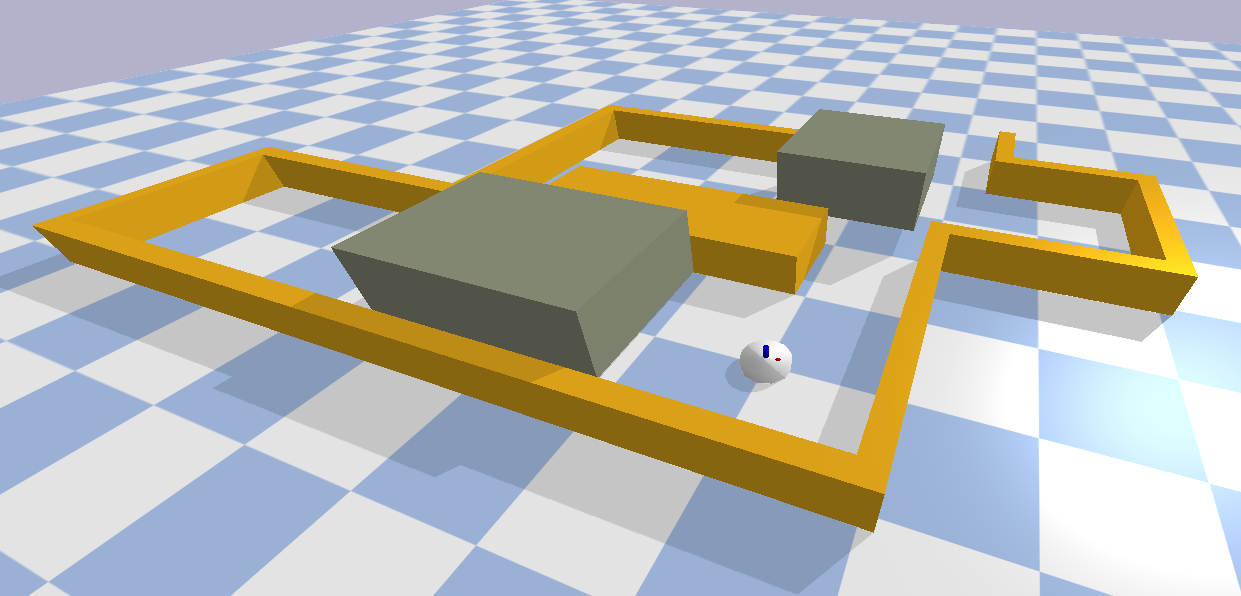
\includegraphics[width=0.9\textwidth]{figures/required_background/planning/two_push_to_freedom_env}
    \caption{Environment with the point robot, unmovable yellow walls and movable brown boxes. Initially the robot classifies all boxes as inkown since it is not provided information weither the walls and boxes are moveable or unmovable.}%
    \label{fig:two_pushes_to_freedom_env}
\end{figure}

The point robot has a cylindrical shape thus a 2-dimensional configuration space is created and can be seen in \Cref{fig:two_pushes_to_freedom_conf_space}.

\begin{figure}[H]
  \centering
  \begin{subfigure}{.49\textwidth}
    \centering
    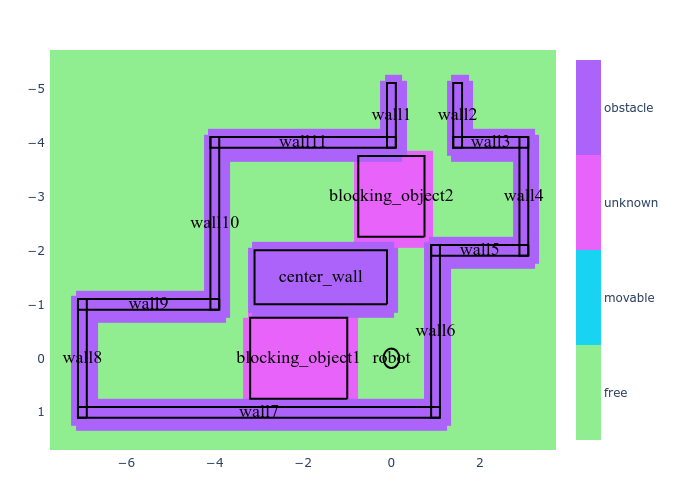
\includegraphics[width=1.05\textwidth]{figures/required_background/planning/c_space_point_robot_grid_size_0_1}
    \caption{$\gls{cspace}^{circle}$ with $\gls{cellSize} = 0.1$}%
    \label{fig:c_space_two_pushes_small}
  \end{subfigure}
  \begin{subfigure}{.49\textwidth}
    \centering
    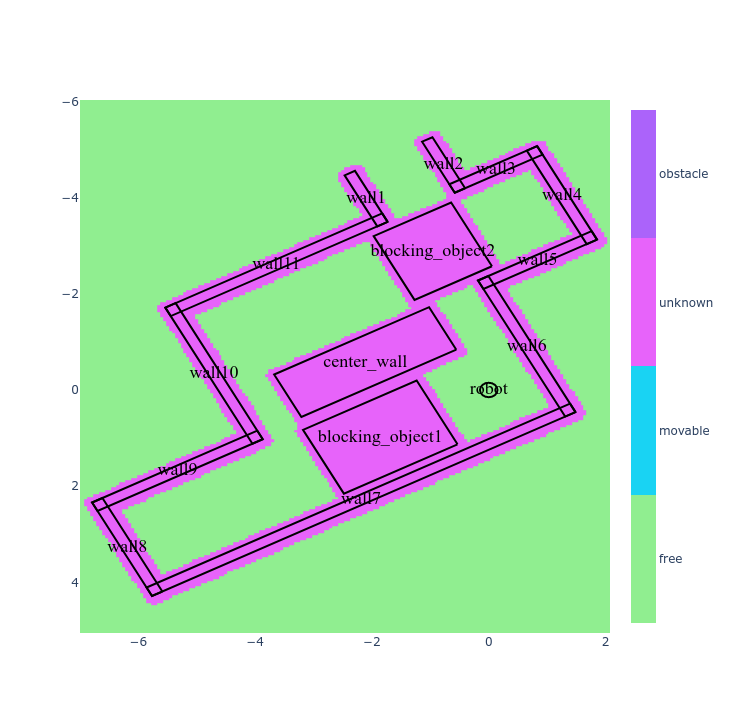
\includegraphics[width=1.05\textwidth]{figures/required_background/planning/c_space_point_robot_grid_size_0_05}
    \caption{$\gls{cspace}^{circle}$ with $\gls{cellSize} = 0.05$}%
    \label{fig:c_space_two_pushes_smaller}
  \end{subfigure}
  \caption{The configuration space for the point robot with different cell sizes. The robot\\environment corresponds to the environment presented in \Cref{fig:two_pushes_to_freedom_env}.}
  \label{fig:two_pushes_to_freedom_conf_space}
\end{figure}

\todo{MARTIJN: I understand what you did here, but you don't explain or illustrate it well. The only difference one can see is the tiny difference at the corners of the walls.}

The resolution of the configuration space at \Cref{fig:c_space_two_pushes_smaller} is higher compared to \Cref{fig:c_space_two_pushes_small} because of the smaller grid size. The difference in resolution is especially visible at the corners of the walls. A high resolution is better at detecting paths through small corridors and tight corners, but it comes at the cost of a longer creation and search time.

\paragraph{Path Existence Algorithm} In the context of this thesis, we can describe path existence as: \textit{For an object's configuration space there exists a list of neighboring cells from starting to target configuration that does not lie in obstacle space.\bs}

A path in configuration space is detected using the implemented\\$f_\mathit{shortest\_path}(\gls{c}_\mathit{start}, \gls{c}_\mathit{target}, \mathit{detect\_blocking\_objects})$ function. This function returns the shortest path from the $\gls{c}_\mathit{start}$ to the $\gls{c}_\mathit{target}$. \textit{detect\_blocking\_objects} is a boolean flag that if \textit{True} returns a list blocking objects that are classified as movable or unknown. If no path can be found, the $f_\textit{shortest\_path}$ function raises an error.\bs

The \textit{shortest\_path} function uses the Dijkstra algorithm~\cite{dijkstra_note_1959} on the discretizing configuration space to find a shortest path. This path can be converted to provide an initial number of samples for motion or manipulation planner, also referred to as a \quotes{warm start}.\bs

\paragraph{Unfeasible solutions and an undecidable problem}
The path estimation algorithm does not take system constraints into account. It is thus possible that the path estimation algorithm finds a list of neighboring cells from the start to the target configuration and concludes that there exists a path. In reality, this path is unfeasible. An example is driving the boxer robot displayed in \Cref{subfig:example_boxer_robot} through a narrow, sharp corner. Whilst geometrically the robot would fit through the corner, the nonholonomic constraints of the robot prevent it from steering through such a tight corner. It is for the motion or manipulation planner to detect that the path is unfeasible.\\

The path estimator suffers from another drawback, finding proof that there exists a path that is undecidable~\cite{zhang_simple_2008}. This is due to the chosen cell size during discretizing the configuration space. An example is a corridor that has exactly the width of the robot, the robot does fit exactly through this corridor. Detecting such a path requires a number of neighboring cells that lie exactly in the center line of the corridor. Only with a cell size going to zero, and the number of cells going to infinity such a path is guaranteed to be detected. Path non-existence on the other hand is more easily to proof, because the path estimation algorithm provides an upper bound on existing paths and a lower bound on non-existing paths~\cite{zhang_simple_2008}.\bs

The path existence algorithm can detect non-existence paths. Thus checking path existence before motion or manipulation planning filters out several non-existent paths that would otherwise waste time and resources. Even if in exceptional cases the path estimation algorithm can yield unfeasible paths and can fail to detect existing paths. Checking path existence before motion or manipulation planning filters a number of non-exist paths and is additionally motivated by two reasons. First, path estimation is orders of magnitude faster compared to motion or manipulation planning. Secondly, the path estimation algorithm can provide a number of initial samples to the motion or manipulation planner that can act as a \quotes{warm start}.

\todo{A path is a list of successive configurations beginning with the start and ending with the target configuration. During planning, constraints are respected by checking the reachability of the configurations added to the path with a system model.}

\subsection{Motion Planning}%
\label{subsec:motion_planning}
Controllers discussed in \Cref{sec:control_methods} can track a path from start to target given that all necessary ingredients are provided. Providing a path is the planners' responsibility, planners seek inside the configuration space for a path from the start to the target configuration. A practical example of such a path is a list of successive points in configurations space, where the first point is the start configuration and the last point is the target configuration. How far the successive points can lie apart is a tuning parameter of the planner. Seeking a path from start to target inside a configuration space whilst avoiding obstacles for the robot to track is referred to as \textit{motion planning}. Finding a path between the start and target configuration for pushing applications whilst avoiding collisions is referred to as \textit{manipulation planning}. This and the upcoming subsection present two new sample-based planners (one for drive, and one for push applications), they are based upon an existing double tree \ac{RRT*} planner~\cite{chen_fast_2018}. The existing planner plans in free and obstacle space, a modification extends the planner to incorporate movable and unknown space. First, this section presents the new motion planning algorithm, and the next section, \Cref{subsec:manipulation_planning} dedicates itself to manipulation planning. The new planning algorithms are sample-based, which can be described as.\bs

\textit{\quotes{The main idea is to avoid the explicit construction of the object space, and instead conduct a search that probes the configuration space with a sampling scheme. This probing is enabled by a collision detection module, which the motion planning algorithm considers as a “black box.”~\cite{lavalle_planning_2006}}}\bs

Generally, the configuration space motion planners plan consists of 2 subspaces, free and obstacle space. The configuration space in this thesis consists of 4 subspaces, namely free, obstacle, unknown and movable space. To solve motion planning problems for such a configuration space a dedicated motion planning algorithm has been developed that extends the existing algorithm extends the existing double tree \ac{RRT*} algorithm~\cite{chen_fast_2018}. The motion planner consists of.

\begin{center}
\begin{align*}
  \gls{nodesMP}:& \textrm{ A set of nodes }\\
  \gls{edgesMP}:& \textrm{ A set of edges }\\
  \gls{pathsMP}:& \textrm{ A set of paths }
\end{align*}
\end{center}

The start connectivity tree consists of the nodes connected by edges containing the starting node, and vice versa for the target connectivity tree containing the target node. The algorithm grows the two \textit{connectivity trees} by randomly sampling configurations and adding them to the start or target connectivity tree. The algorithm explores configuration space by growing these connectivity trees. When the start connectivity tree is close enough (inside the search size of a newly added sample) to the target connectivity tree a path from start to target is found. The goal of the motion planner is to find a path between the start and target configuration that results in the lowest totalPathCost, defined as:

\[\textrm{TotalPathCost} = \textrm{PathCost} + \textrm{MovableSpaceCost} + \textrm{UnknownSpaceCost}\]

The PathCost corresponds to the sum of euclidean distances between the successive configurations in the path, the MovableSpaceCost and UnknownSpaceCost correspond to a fixed addition cost for a configuration in the path crosses through movable or unknown subspace respectively. Here crossing through is defined as one or more nodes in the path lying in that subspace. If a path does not contain a node in movable space, MovableSpaceCost will be 0, equivalent to unknown space and UnknownSpaceCost. By optimizing the path for the lowest cost the motion planning algorithm is incentivized to find a path around unknown or movable objects. However, if there is no path in free space only, the algorithm plans through movable or unknown space. Newly sampled configurations are added in a structural manner that guarantees an optimal path is found with infinite sampling~\cite{chen_fast_2018}. Where optimality is defined as the path with the lowest possible cost.\bs

\paragraph{Tuning Parameters}
The algorithm has 4 tuning parameters that can be tweaked, first, the \textit{step size}, the maximal normalized distance between connected samples in the connectivity trees, see \Cref{subfig:mp_step_size} for a visual example. Choosing a high step size will increases the search speed because the connectivity trees grow faster. A higher step size comes at the cost of smoothness, the resulting path will be bumpier with sharper corners. Additionally, the path has an increased chance of collision with obstacles because, for two connected configurations in a path, the individual configurations can both lie in free space. The space between configurations is not checked and an obstacle could be in between the configurations, especially when cutting corners around obstacles. The second tuning parameter is the \textit{search size}, which is a subspace around the newly sampled sample (see, \Cref{subfig:mp_search_size}). In this subspace, a parent node is sought and rewiring occurs. A new node is connected with an edge to a connectivity tree through a parent node. After connecting the new node to its parent node, rewiring occurs which is changing the parent node by removing and adding an edge if that results in a lower cost for that node, rewiring can be visually seen in \Cref{subfig:mp_rewire}. Increasing the search size improves the choice of parent node and improves cost due to rewiring, but it also exponentially increases computation time. The third and fourth tuning parameters are the fixed costs for crossing through movable or unknown space, \Cref{fig:mp_push_or_drive} clearly shows the effect of varying such costs.\bs

Pseudocode of the proposed algorithm is provided in \Cref{pseudocode:proposed_rrt_star}. The functions used are elaborated upon in the following \Cref{table:functions_for_proposed_rrt_star}.\bs


\noindent
\begin{table}[H]
  \centering
  \begin{tabular}%
  {>{\raggedright\arraybackslash}p{0.25\textwidth}%
   >{\raggedright\arraybackslash}p{0.65\textwidth}}
  $x$:& A node representing a point in configuration space\\
  $x_{init}$:& Creates a start and target node\\ 
  \textit{NotReachStop}:& True if the stopping criteria is not reached\\ 
  $\mathit{Sample_{random}}$:& Creates a random sample in free-, movable- or unknown space\\
  $\mathit{Nearest}(x, V)$:& Returns the nearest nodes from $x$ in $V$\\
  $\mathit{NearestSet}(x, V)$:& Returns set of nearest nodes from $x$ in $V$\\
  $\mathit{Project}(x, x')$:& Project $x$ toward $x'$\\
  $\mathit{CollisionCheck}(x)$:& Returns true if $x$ is in free-, movable- or unknown space\\
  $\mathit{ObjectCost}(x', x)$:& Returns a fixed additional cost if $x$ enters movable- or unknown space from $x'$, otherwise returns 0\\
  $\mathit{Distance}(x, x')$:& Returns the distance between sample $x$ and $x'$\\
  $\mathit{CostToInit}(x)$:& Find the total cost from $x$ to the initial node\\
    $\mathit{ReachabilityCheck}(x, x')$:& Return true if a system model with initial state $x$ is able to reach state $x'$ for a range of allowed input, otherwise, return false.\\
    $\mathit{InSameTree}(x, x')$:& Returns true if both $x$ and $x'$ are in the same tree, otherwise return false\\
  \end{tabular}
\caption{Functions used by the \Cref{pseudocode:proposed_rrt_star}}
\label{table:functions_for_proposed_rrt_star}
\end{table}

Notice that in \Cref{pseudocode:proposed_rrt_star} the colored sections correspond to the surrounding colored border in the subfigures of \Cref{fig:motion_planner_adding_one_sample}.\bs

\newpage
\begin{algorithm}[H]
\caption{Pseudocode for modified double tree \ac{RRT*} algorithm}%
\label{pseudocode:proposed_rrt_star}
\begin{algorithmic}[1]

\hspace{-0.9cm}\colorbox{my_grey}{\parbox{\linewidth}{%
\State $\gls{nodesMP} \leftarrow x_{init}$
\While{\textit{NotReachStop}} 

\hspace{-0.1cm}\colorbox{my_light_blue}{\parbox{\linewidth}{%
    \State $Cost_\mathit{min} \leftarrow +\infty$ \algorithmiccomment{Create, check and project a new random sample}
    \State $\gls{nodeMP}_\mathit{rand} \leftarrow \mathit{Sample_{random}}$
    \State $\gls{nodeMP}_\mathit{nearest} \leftarrow \mathit{Nearest(\gls{nodeMP}_{rand}, \gls{nodesMP})}$
    \State $\gls{nodeMP}_\mathit{temp} \leftarrow \mathit{Project(\gls{nodeMP}_{rand}, \gls{nodeMP}_{nearest})}$

    \If{$\mathit{CollisionCheck(\gls{nodeMP}_{temp})}$}
    \State $\gls{nodeMP}_\mathit{new} = \gls{nodeMP}_\mathit{temp}$
    \Else
        \State Continue
    \EndIf
}}

\hspace{-0.1cm}\colorbox{my_yellow}{\parbox{\linewidth}{%
    \State $X_\mathit{near} \leftarrow \mathit{NearestSet(\gls{nodeMP}_{new}, \gls{nodesMP})}$ \algorithmiccomment{Find and connect new node to parent node}
    \For{$\gls{nodeMP}_\mathit{near} \in X_\mathit{near}$}
    \State $\mathit{Cost_{temp}} \leftarrow \mathit{CostFromInit(\gls{nodeMP}_{near}) + Distance(\gls{nodeMP}_{near}, \gls{nodeMP}_{new}) + ObjectCost(\gls{nodeMP}_{near}, \gls{nodeMP}_{new})}$
    \If{$\mathit{Cost_{temp}}  < \mathit{Cost_{min}}$}
    \If{$\mathit{ReachabilityCheck(\gls{nodeMP}_{new}, \gls{nodeMP}_{near})}$}
    \State $\mathit{Cost_{min}} \leftarrow \gls{nodeMP}_\mathit{temp}$
    \State $\gls{nodeMP}_\mathit{minCost} \leftarrow \gls{nodeMP}_\mathit{near}$
            \EndIf
        \EndIf
    \EndFor
    \If{$\mathit{Cost_{min}} == \infty$}
        \State Continue
    \Else
    \State $\gls{nodesMP}.add(\gls{nodeMP}_\mathit{new})$
    \State $E.\mathit{add}(\gls{nodeMP}_\mathit{minCost}, \gls{nodeMP}_\mathit{new})$
    \EndIf
}}

\hspace{-0.1cm}\colorbox{my_green}{\parbox{\linewidth}{%
    \State $\mathit{Cost_{path}} \leftarrow +\infty$ \algorithmiccomment{Check if the newly added node can lower cost for nearby nodes}
    \For{$\gls{nodeMP}_\mathit{near} \in X_{near}$} 
    \If{$\mathit{InSameTree(\gls{nodeMP}_{near}, \gls{nodeMP}_{new})}$} 
    \State $\mathit{Cost_{temp}} \leftarrow \mathit{CostFromInit(\gls{nodeMP}_{new}) + distance(\gls{nodeMP}_{new}, \gls{nodeMP}_{near}) + ObjectCost(\gls{nodeMP}_{new}, \gls{nodeMP}_{near})}$
    \If{$\mathit{Cost_{temp} < CostFromInit(\gls{nodeMP}_{near})}$}
    \If{$\mathit{ReachabilityCheck(\gls{nodeMP}_{new}, \gls{nodeMP}_{near})}$}
    \State $\mathit{E.rewire(\gls{nodeMP}_{near}, \gls{nodeMP}_{new})}$
           \EndIf
        \EndIf
      \Else \algorithmiccomment{Add lowest cost path to the list of paths}
      \State $\mathit{Cost_{temp} \leftarrow CostFromInit(\gls{nodeMP}_{new}) + distance(\gls{nodeMP}_{new}, \gls{nodeMP}_{near})} $ \newline\hspace*{10em} $+ \mathit{CostFromInit(\gls{nodeMP}_{near}) + ObjectCost(\gls{nodeMP}_{new}, \gls{nodeMP}_{near})}$
          \If{$\mathit{Cost_{temp}  < Cost_{path}}$}
          \If{$\mathit{ReachabilityCheck(\gls{nodeMP}_{new}, \gls{nodeMP}_{near})}$}
          \State $\mathit{Cost_{pathMin} \leftarrow \gls{nodeMP}_{temp}}$
          \State $\mathit{\gls{nodeMP}_{pathMin} \leftarrow \gls{nodeMP}_{near}}$
              \EndIf
          \EndIf
      \EndIf
      \If{$Cost_{pathMin} == \infty$}
          \State Continue
      \Else
      \State $\mathit{P.addPath(\gls{nodeMP}_{new}, \gls{nodeMP}_{pathMin}, Cost_{pathMin})}$
      \EndIf
    \EndFor
}}
\EndWhile
}}
\end{algorithmic}
\end{algorithm}

\newpage
Now an example is provided of the proposed algorithm, see \Cref{fig:motion_planner_adding_one_sample}. In this example, one single sample is added to the starting connectivity tree. Adding this sample involves many steps, which are generating a new random sample, projecting the sample to the nearest node, rewiring nearby samples and connecting the start to the target tree.\bs

\begin{figure}[H]
    \centering
    \begin{subfigure}{.49\textwidth}
    \centering
    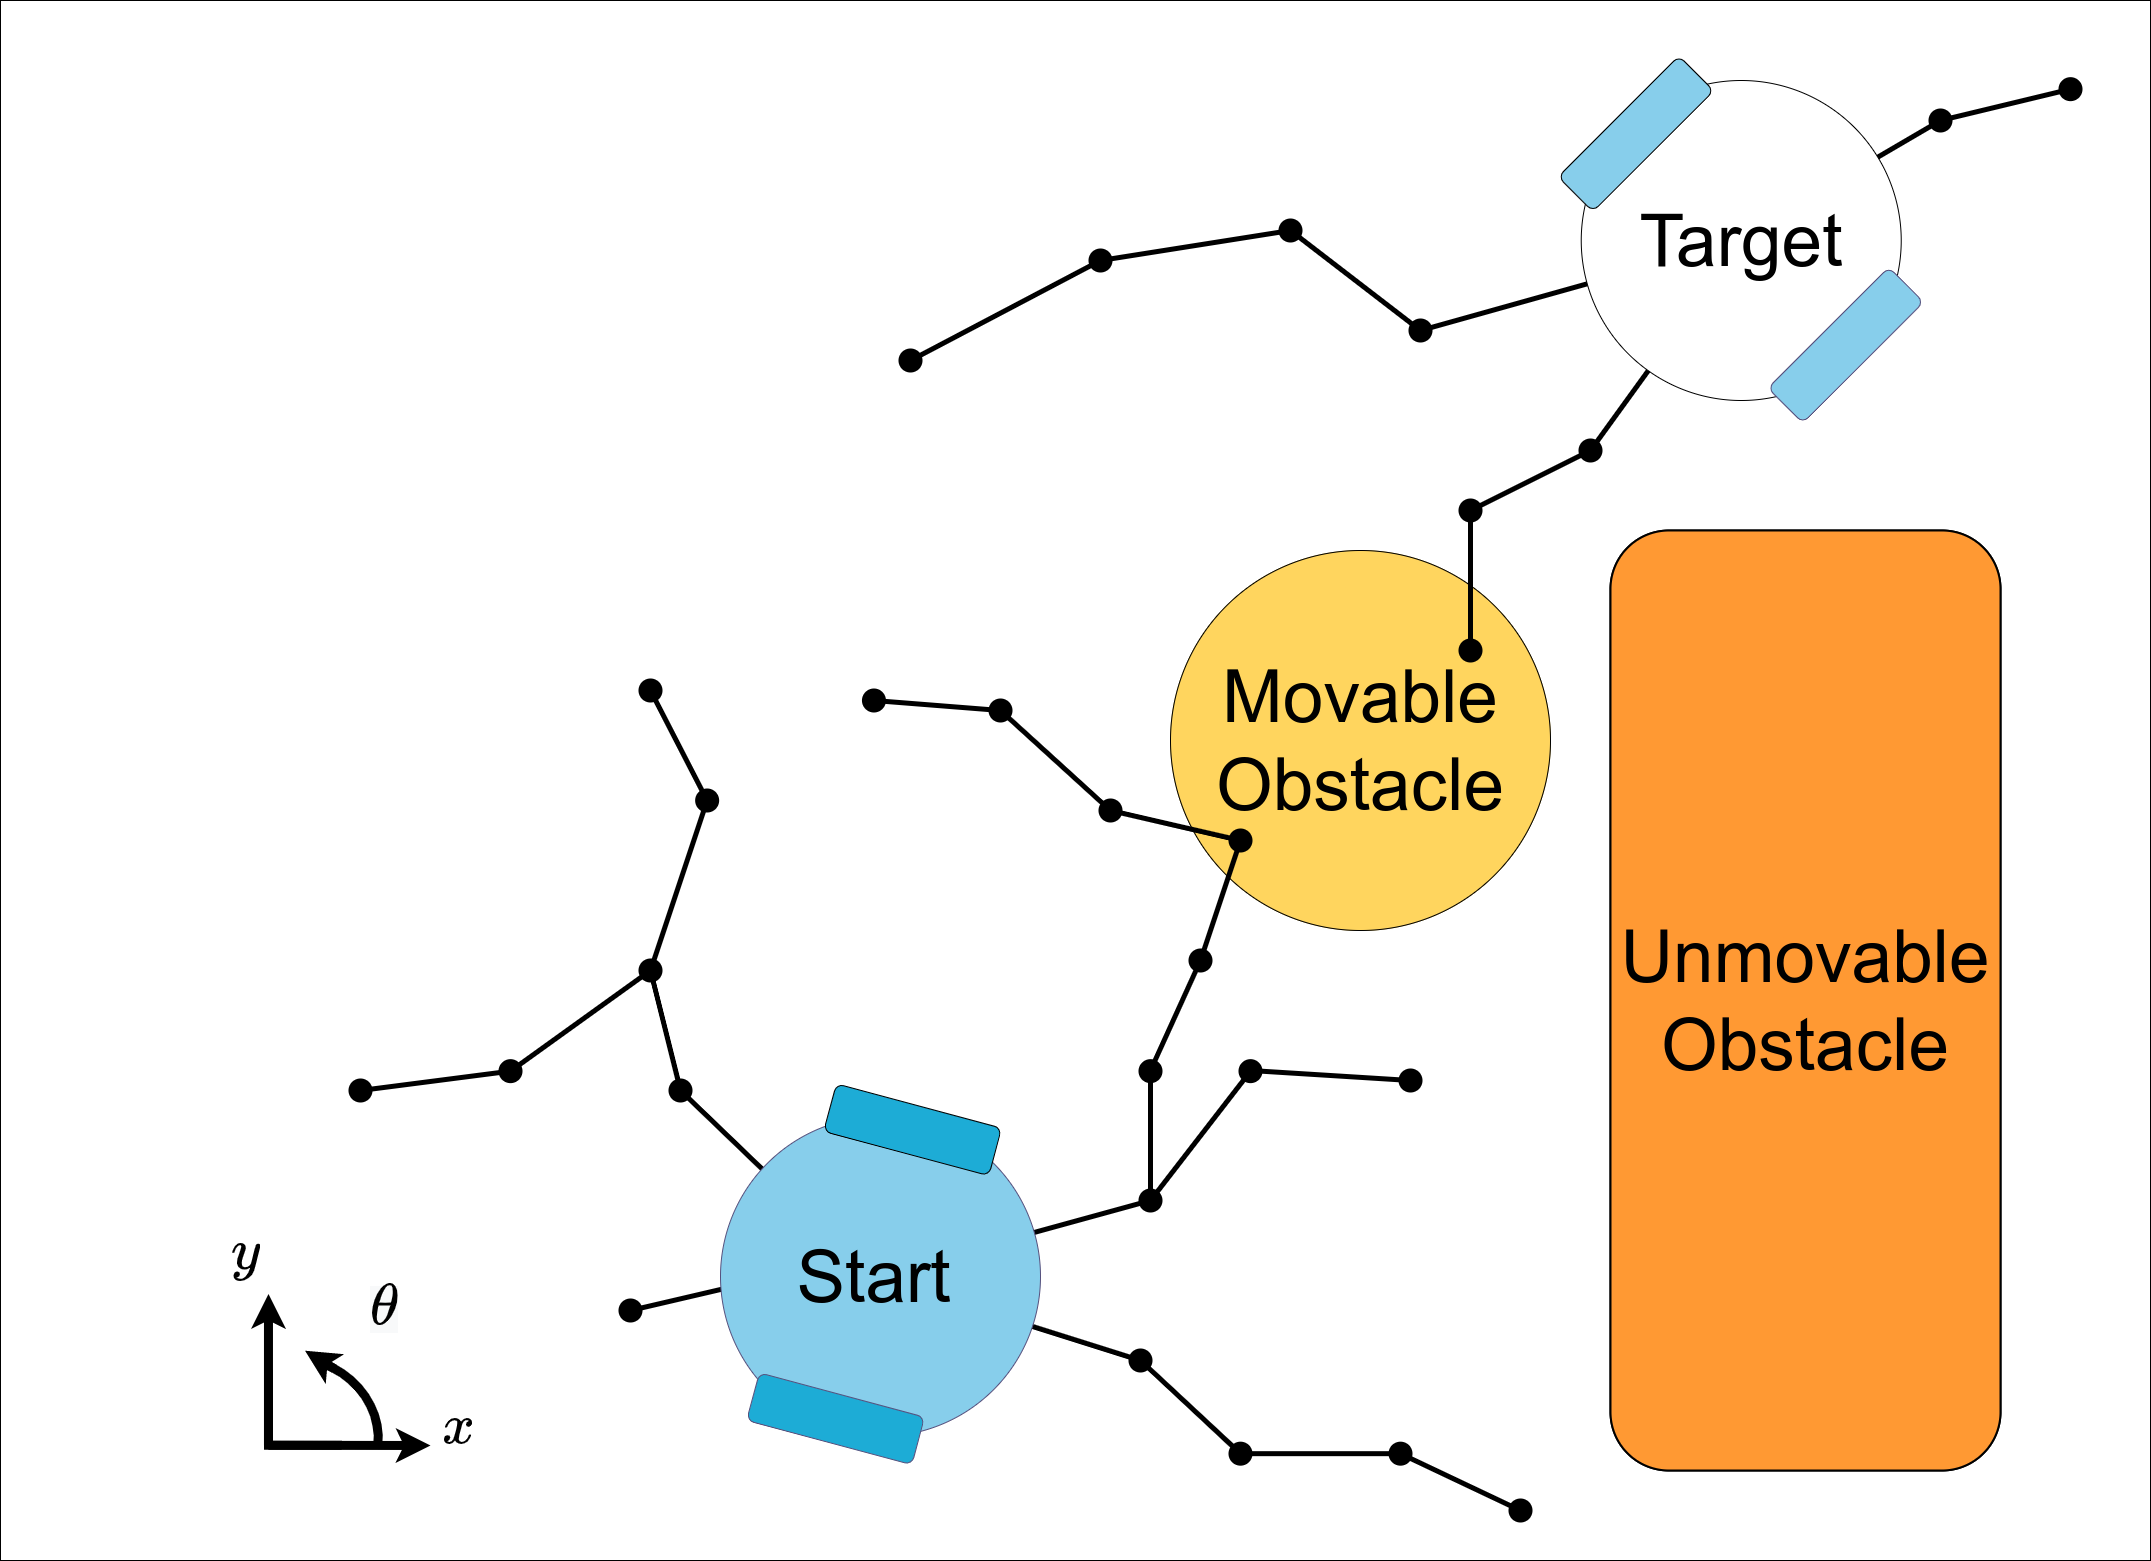
\includegraphics[width=0.93\textwidth, cfbox=my_grey 5pt 0pt]{figures/required_background/mp/1mp_init.drawio.png}
    \caption{Snapshot of the configuration space during a search\\from start to the target configuration.}
    \end{subfigure}
    \begin{subfigure}{.49\textwidth}
    \centering
    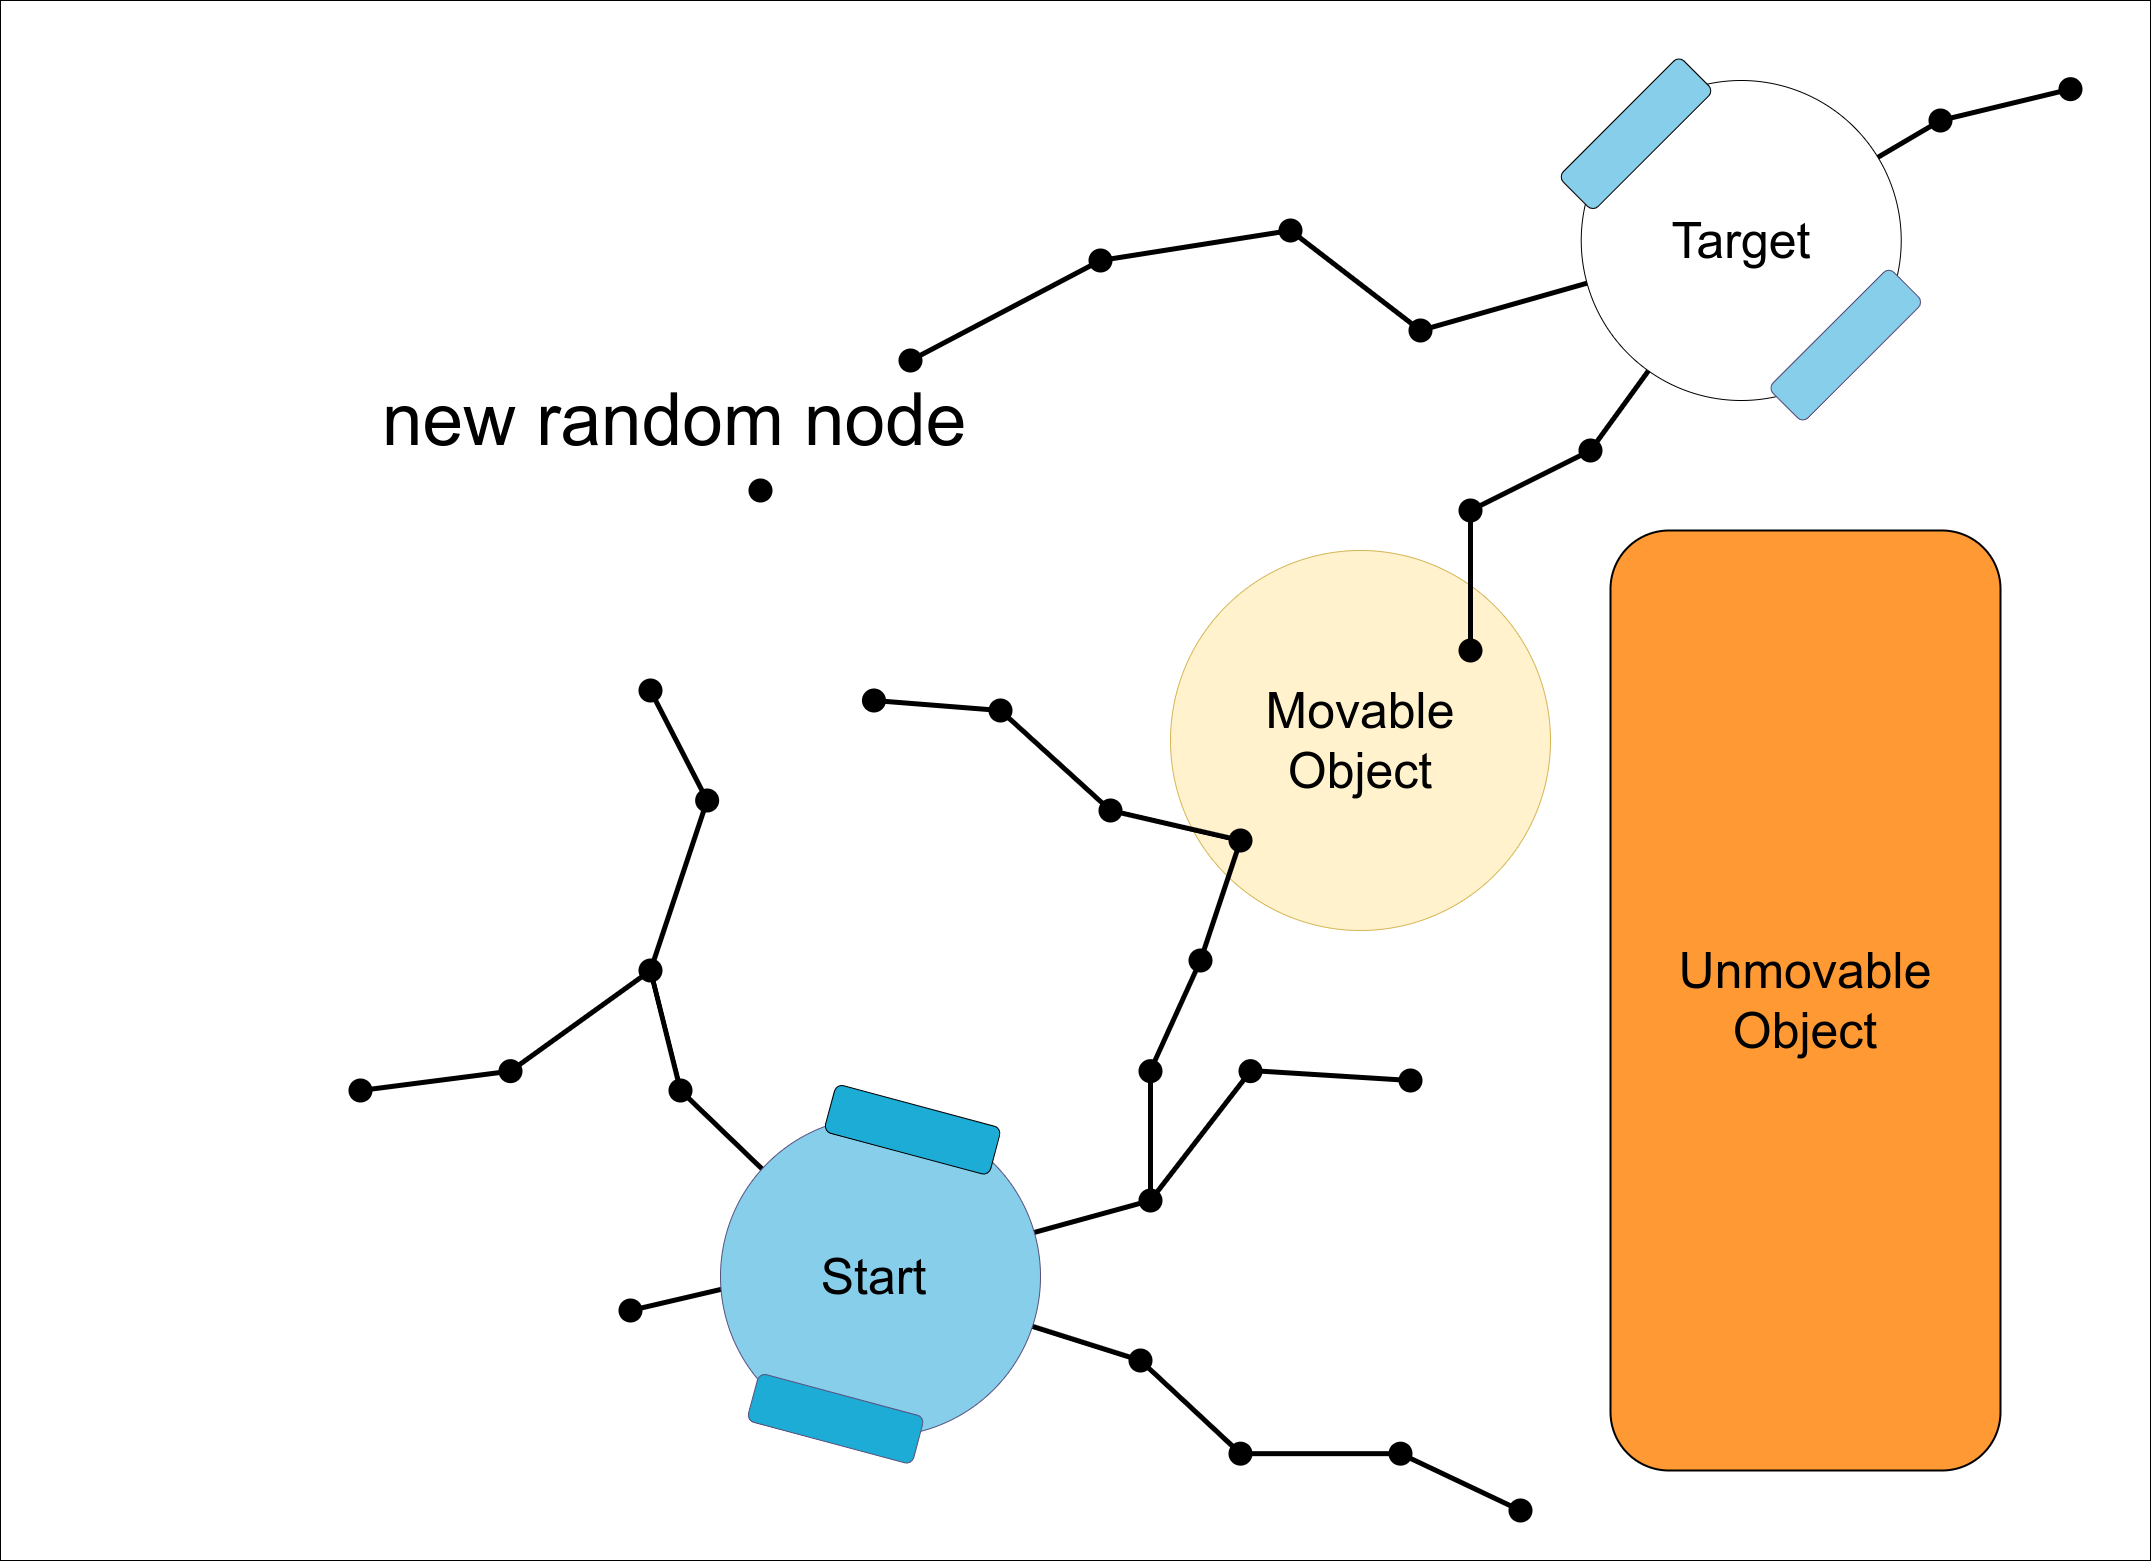
\includegraphics[width=0.93\textwidth, cfbox=my_light_blue 5pt 0pt]{figures/required_background/mp/2mp_new_rand_sample.drawio.png}
    \caption{A new random sample is generated.\newline}
    \end{subfigure}

    \begin{subfigure}{.49\textwidth}
    \centering
    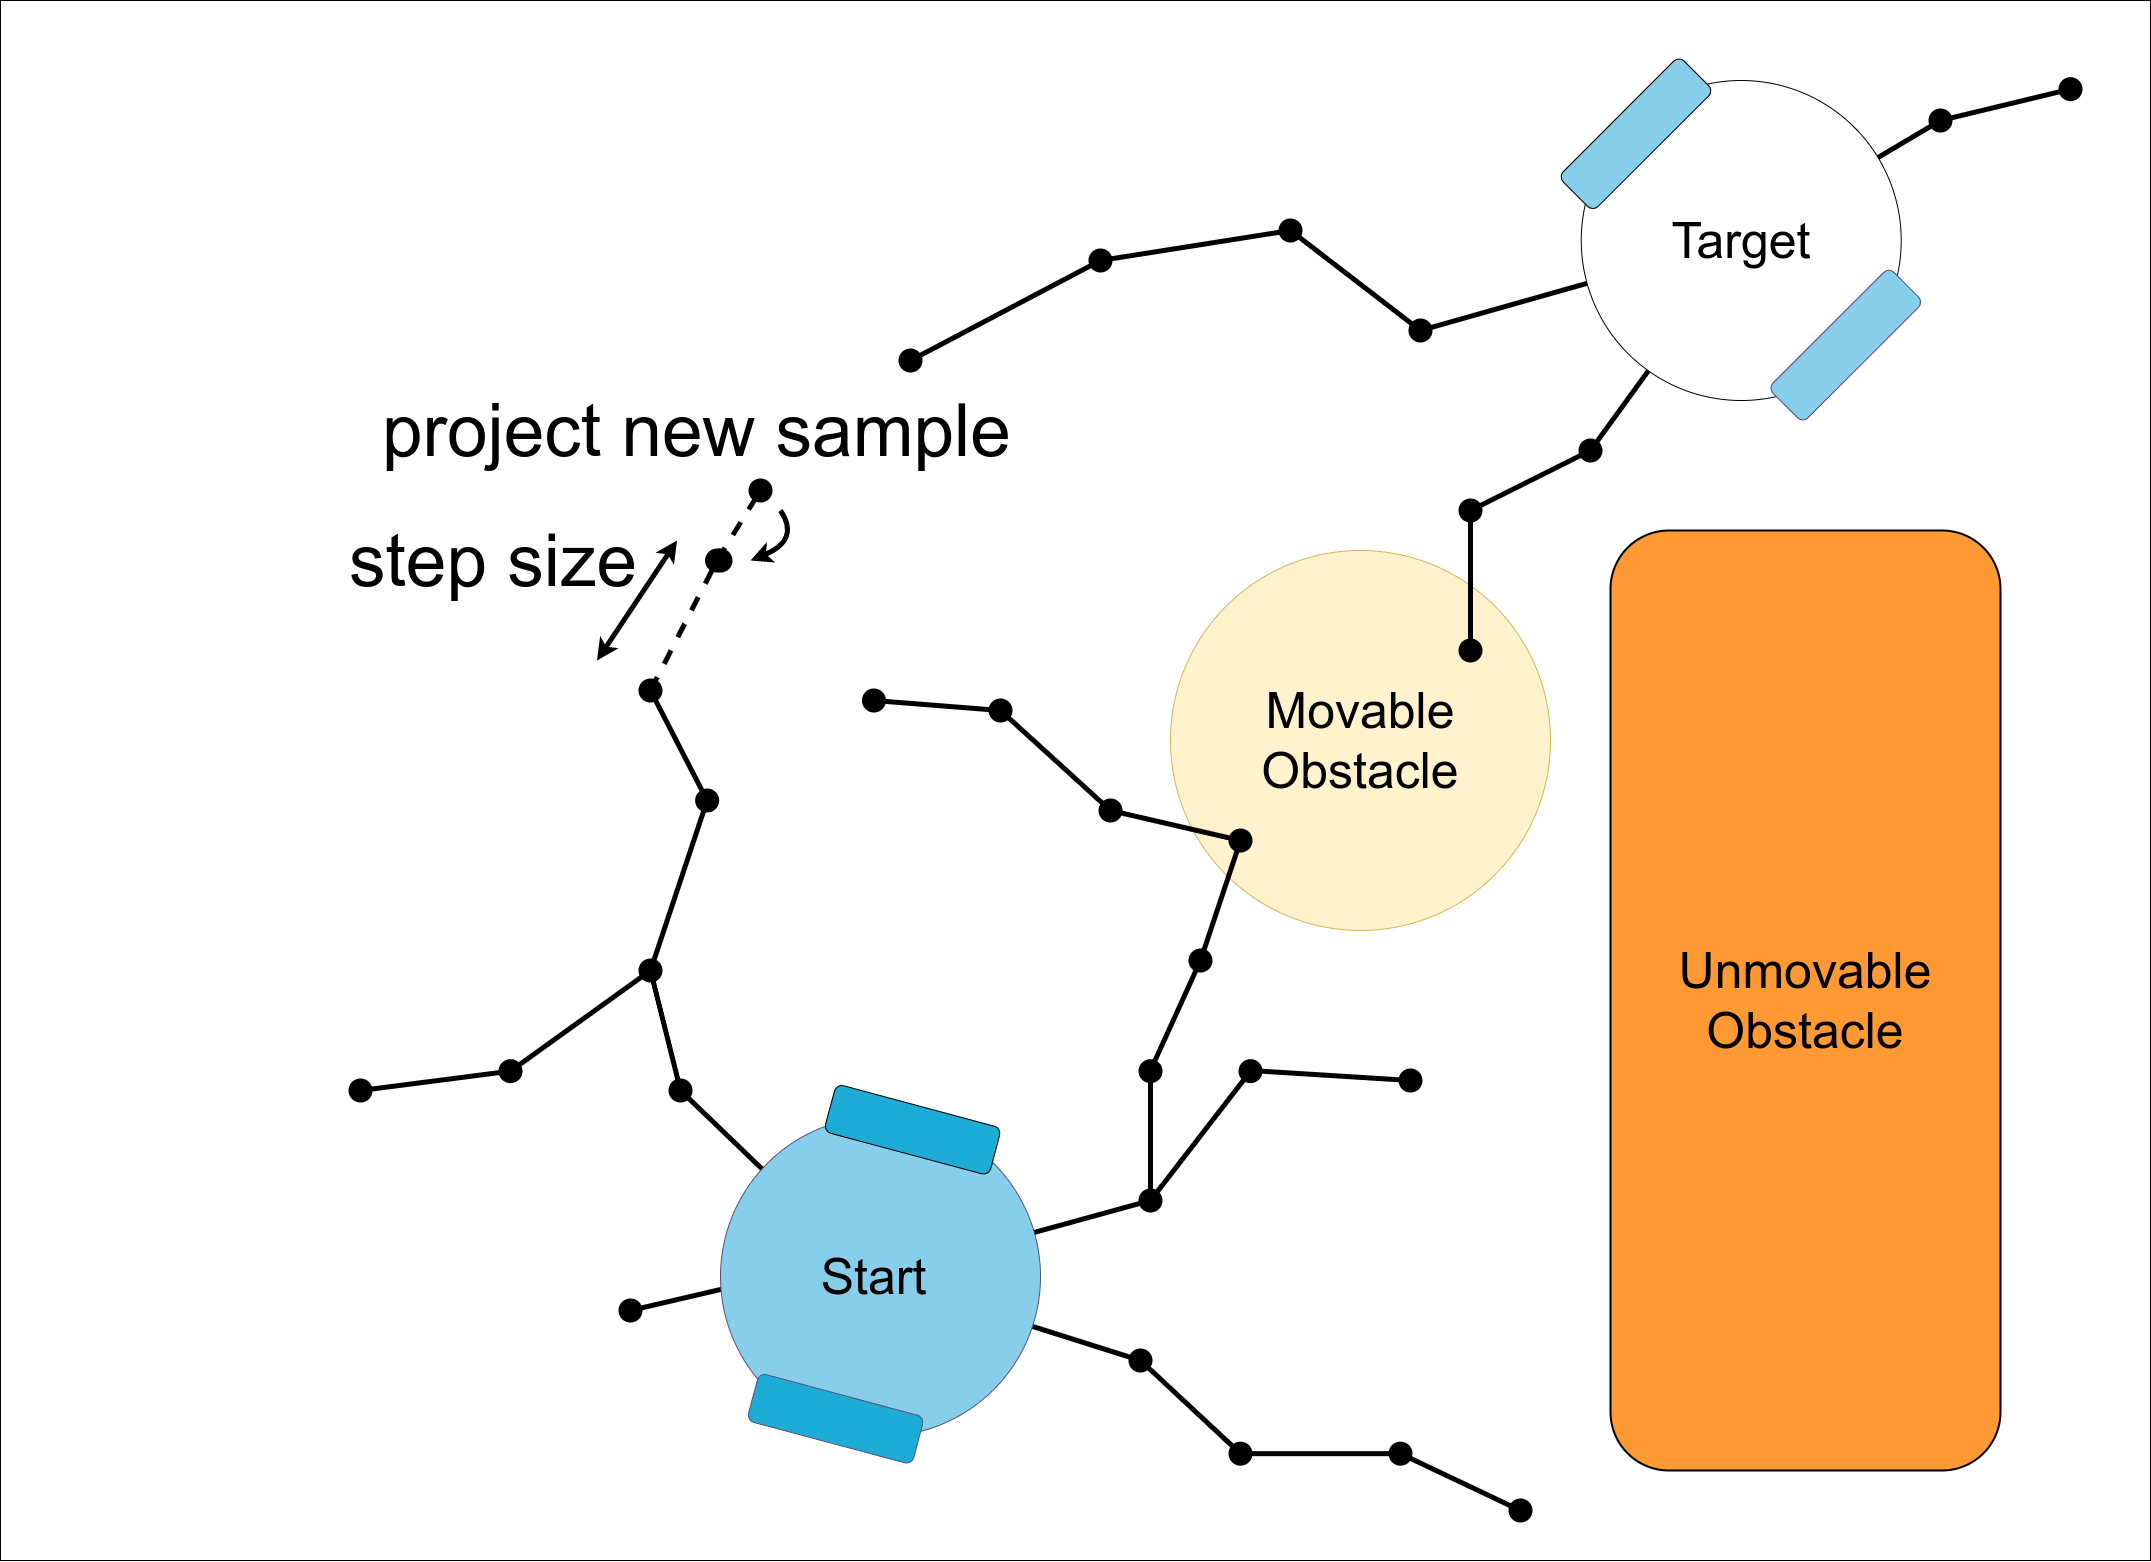
\includegraphics[width=0.93\textwidth, cfbox=my_light_blue 5pt 0pt]{figures/required_background/mp/3mp_project_sample.drawio.png}
    \caption{The new sample is projected toward the closest sample.\bs}%
    \label{subfig:mp_step_size}
    \end{subfigure}
    \begin{subfigure}{.49\textwidth}
    \centering
    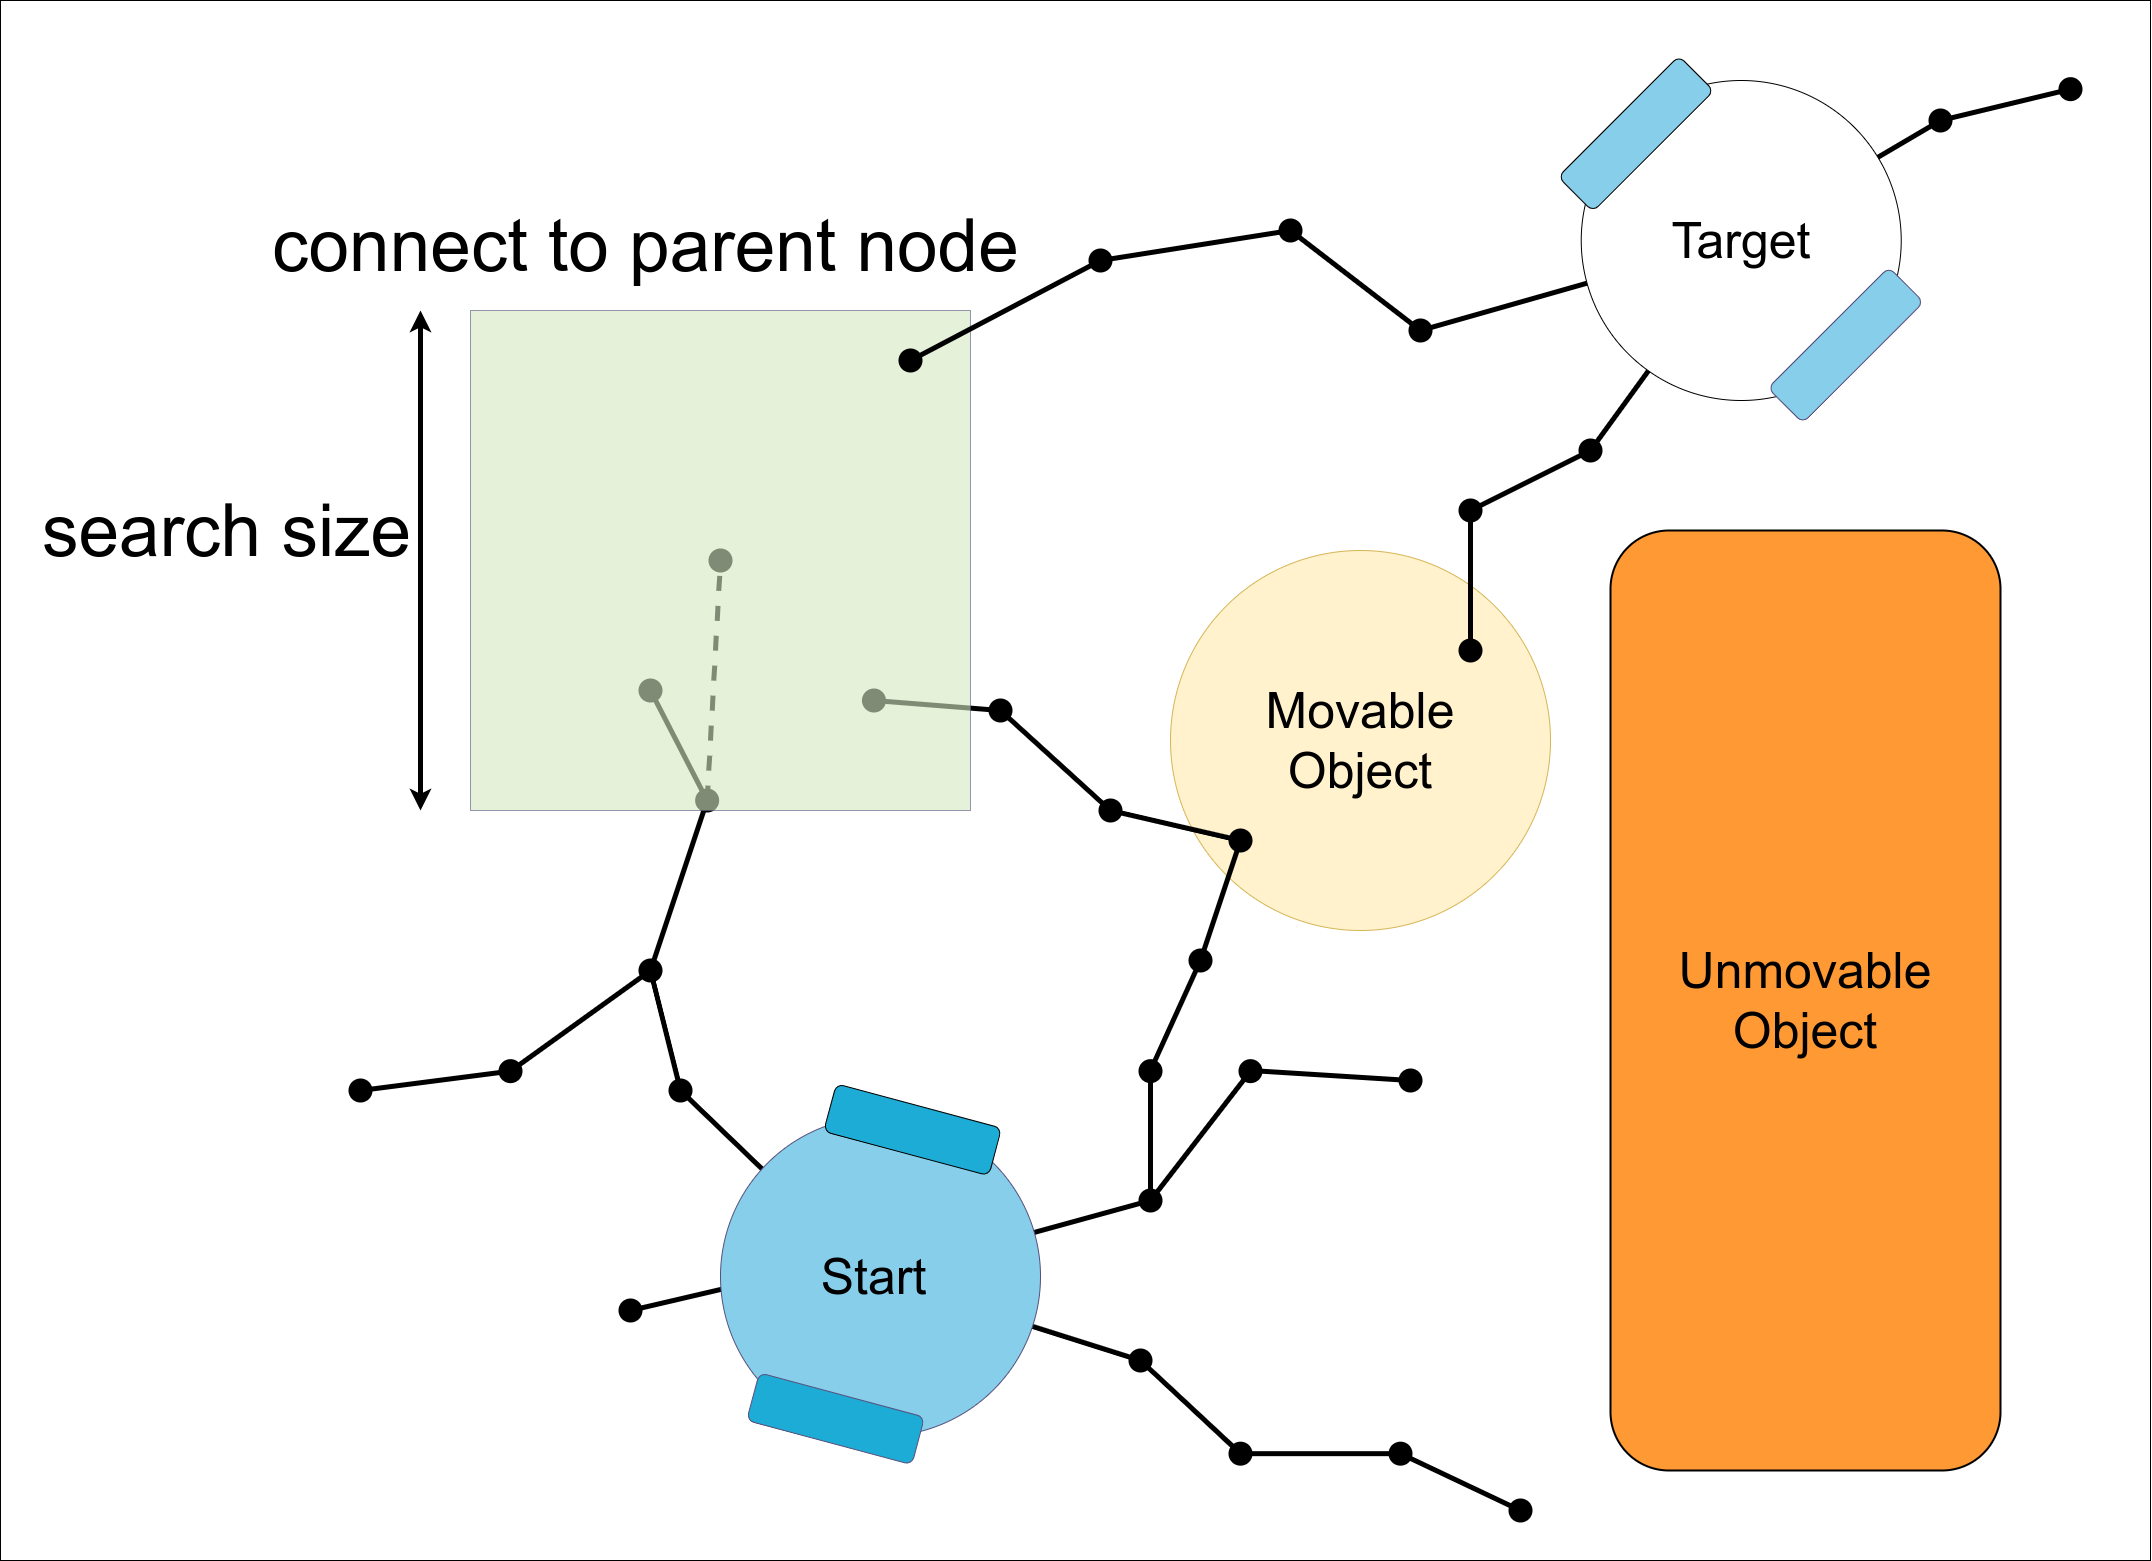
\includegraphics[width=0.93\textwidth, cfbox=my_yellow 5pt 0pt]{figures/required_background/mp/4mp_connect_to_tree.drawio.png}
    \caption{The new sample is connected to the node in search space\\that results in the lowest cost.}%
    \label{subfig:mp_search_size}
    \end{subfigure}

    \begin{subfigure}{.49\textwidth}
    \centering
    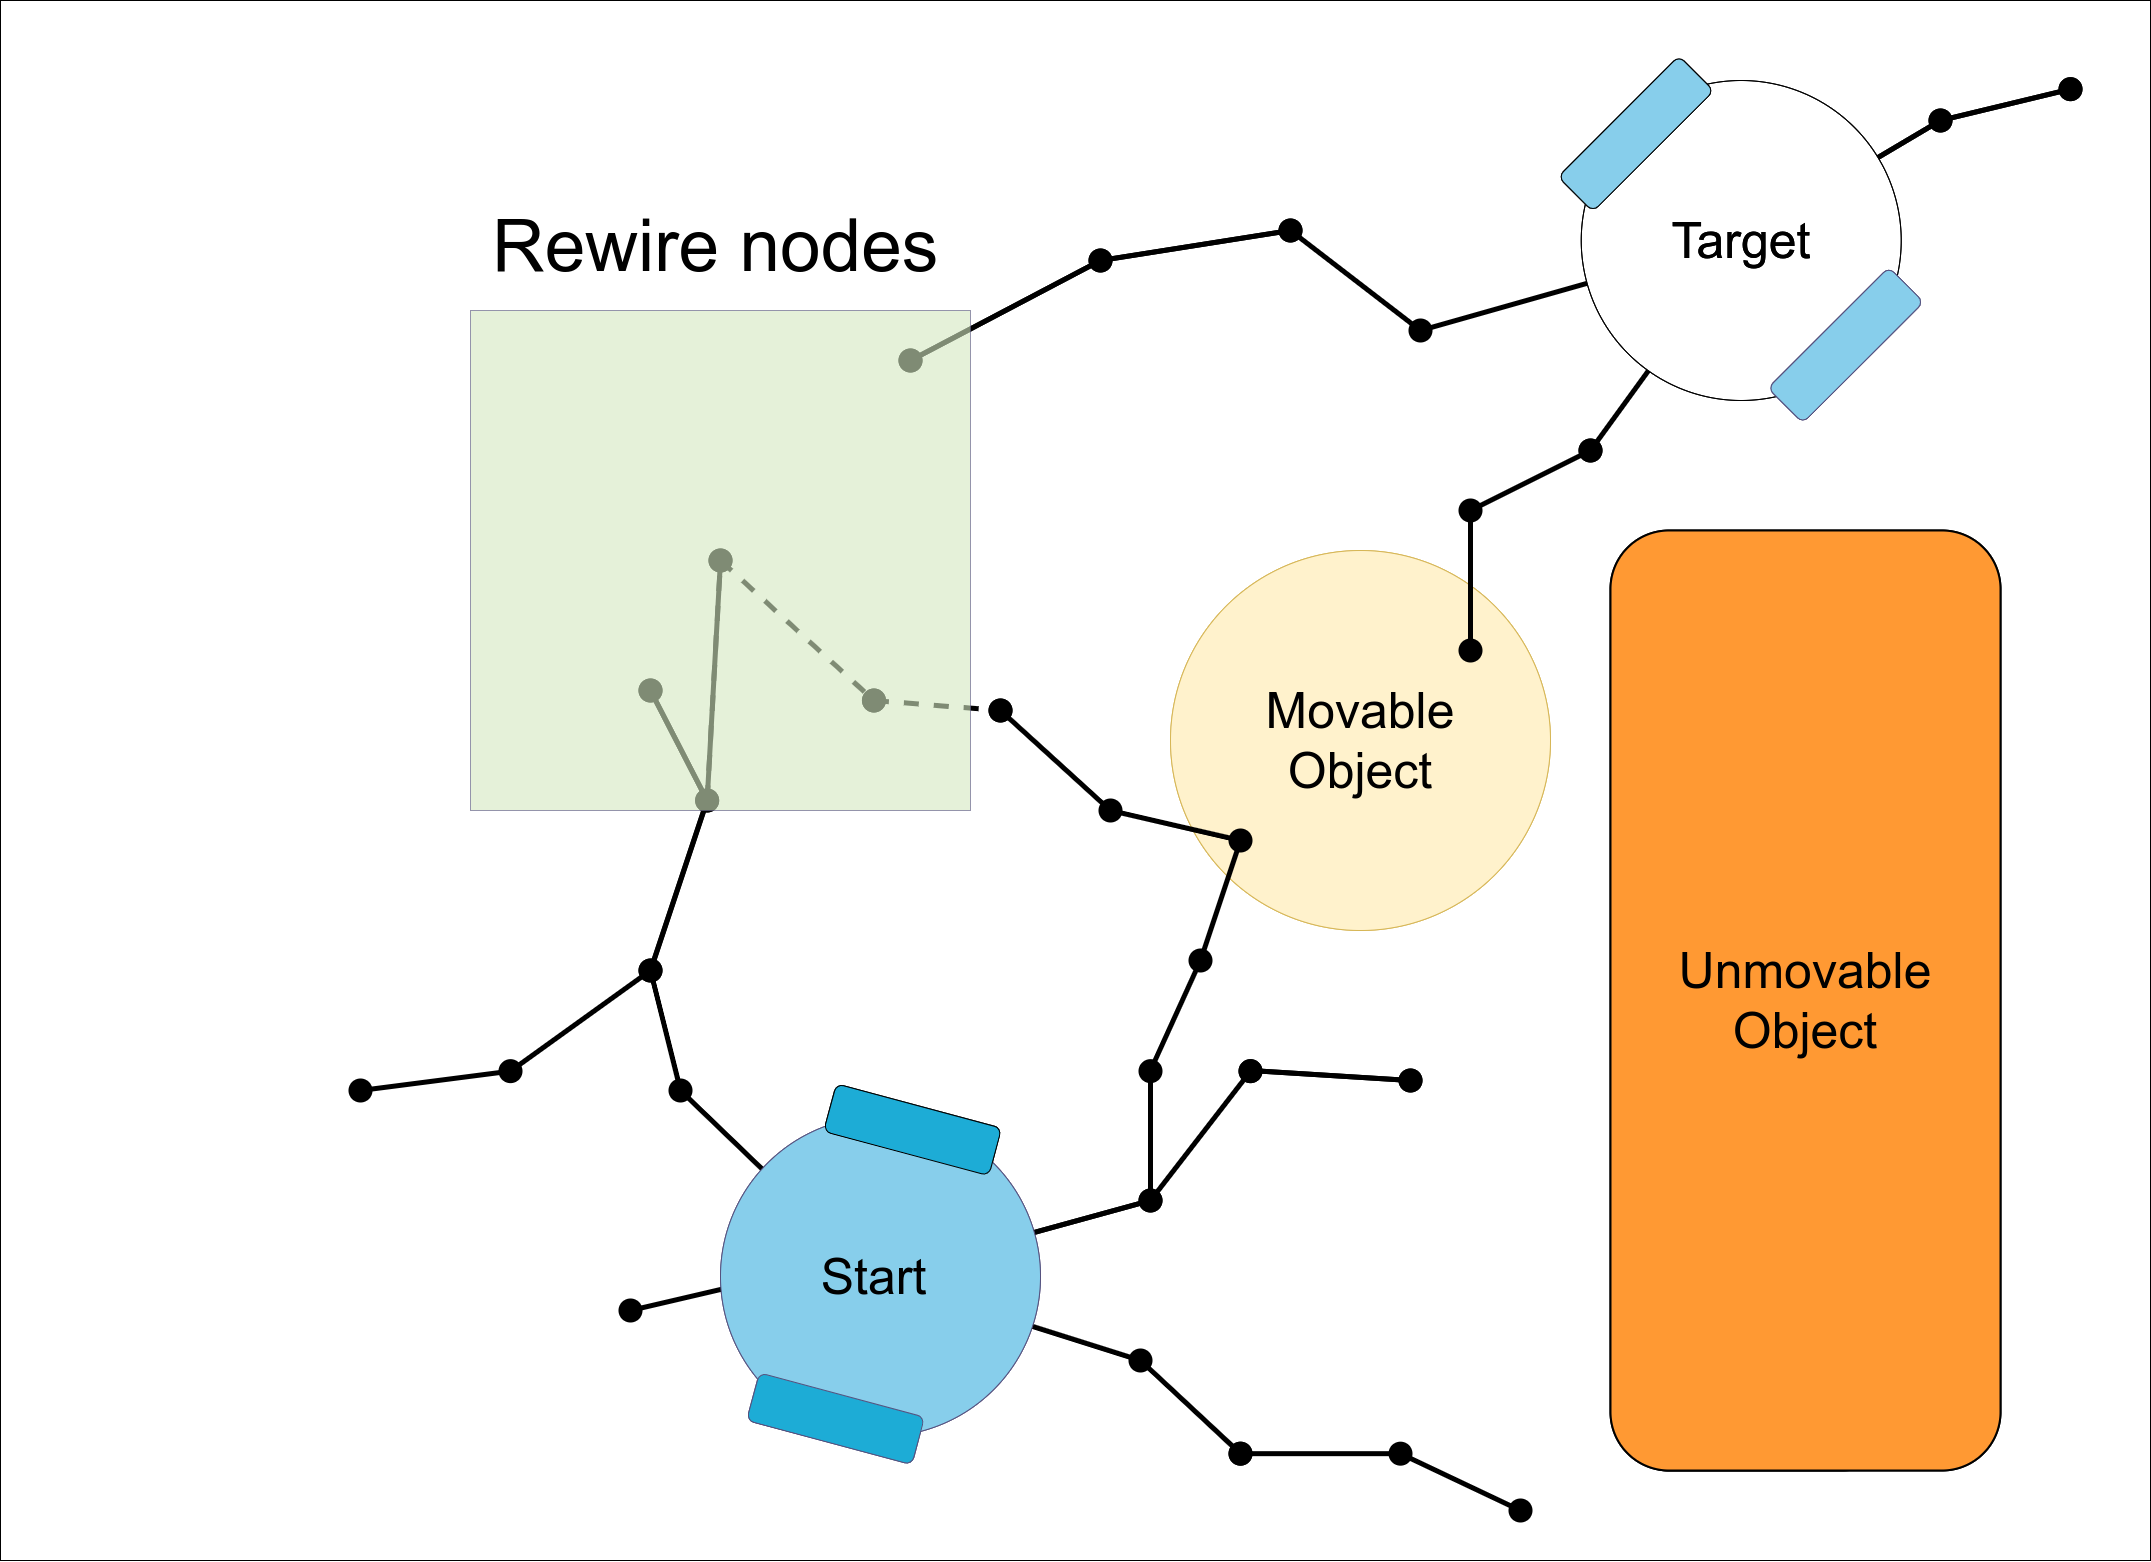
\includegraphics[width=0.93\textwidth, cfbox=my_green 5pt 0pt]{figures/required_background/mp/5mp_rewire.drawio.png}
    \caption{Nodes for which the cost can be lowered\\from the new sample are rewired.}%
    \label{subfig:mp_rewire}
    \end{subfigure}
    \begin{subfigure}{.49\textwidth}
    \centering
    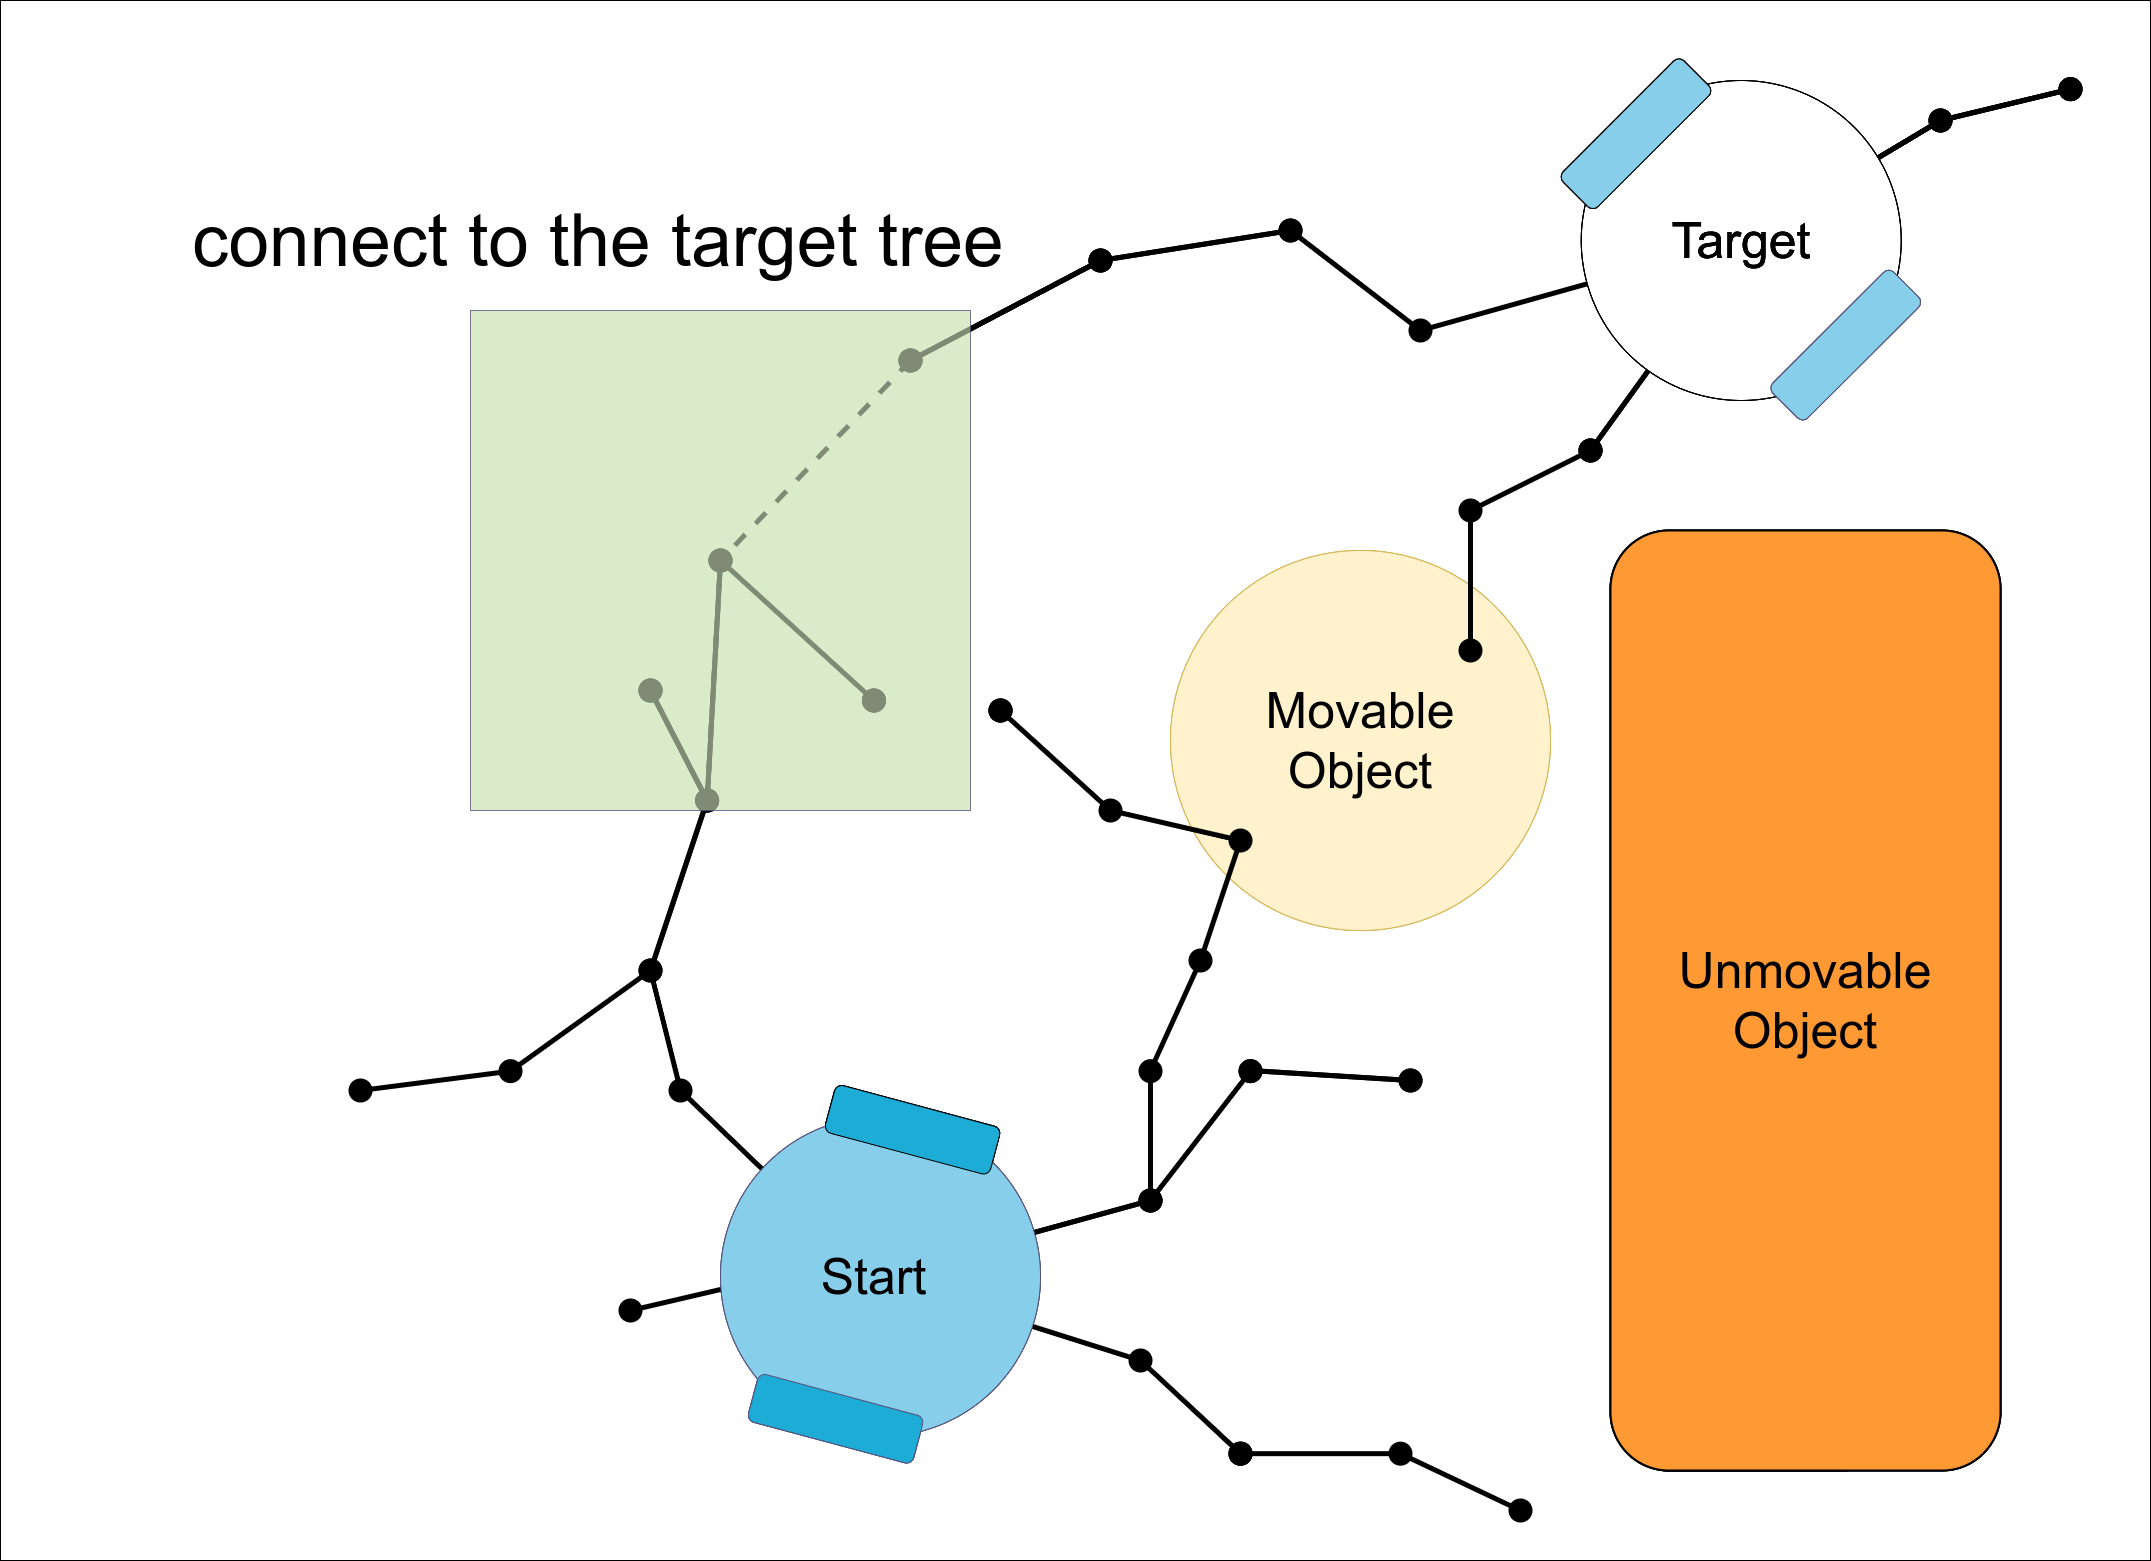
\includegraphics[width=0.93\textwidth, cfbox=my_green 5pt 0pt]{figures/required_background/mp/6mp_search_other_tree.drawio.png}
    \caption{A path from start to target configuration is found. \bs}
    \end{subfigure}

    \caption{Visualization of the Double tree \acs{RRT*} motion planner that adds a single sample to the connectivity graph. The color of the box surrounding subfigures corresponds to the colored sections in \Cref{pseudocode:proposed_rrt_star}. 3-dimensional configuration space displayed as 2-dimensional configuration space ($x$ and $y$ are visible, $\theta$ is not visible).}
    \label{fig:motion_planner_adding_one_sample}
\end{figure}

\begin{figure}[H]
    \centering
    \begin{subfigure}{0.5\textwidth}
    \centering
    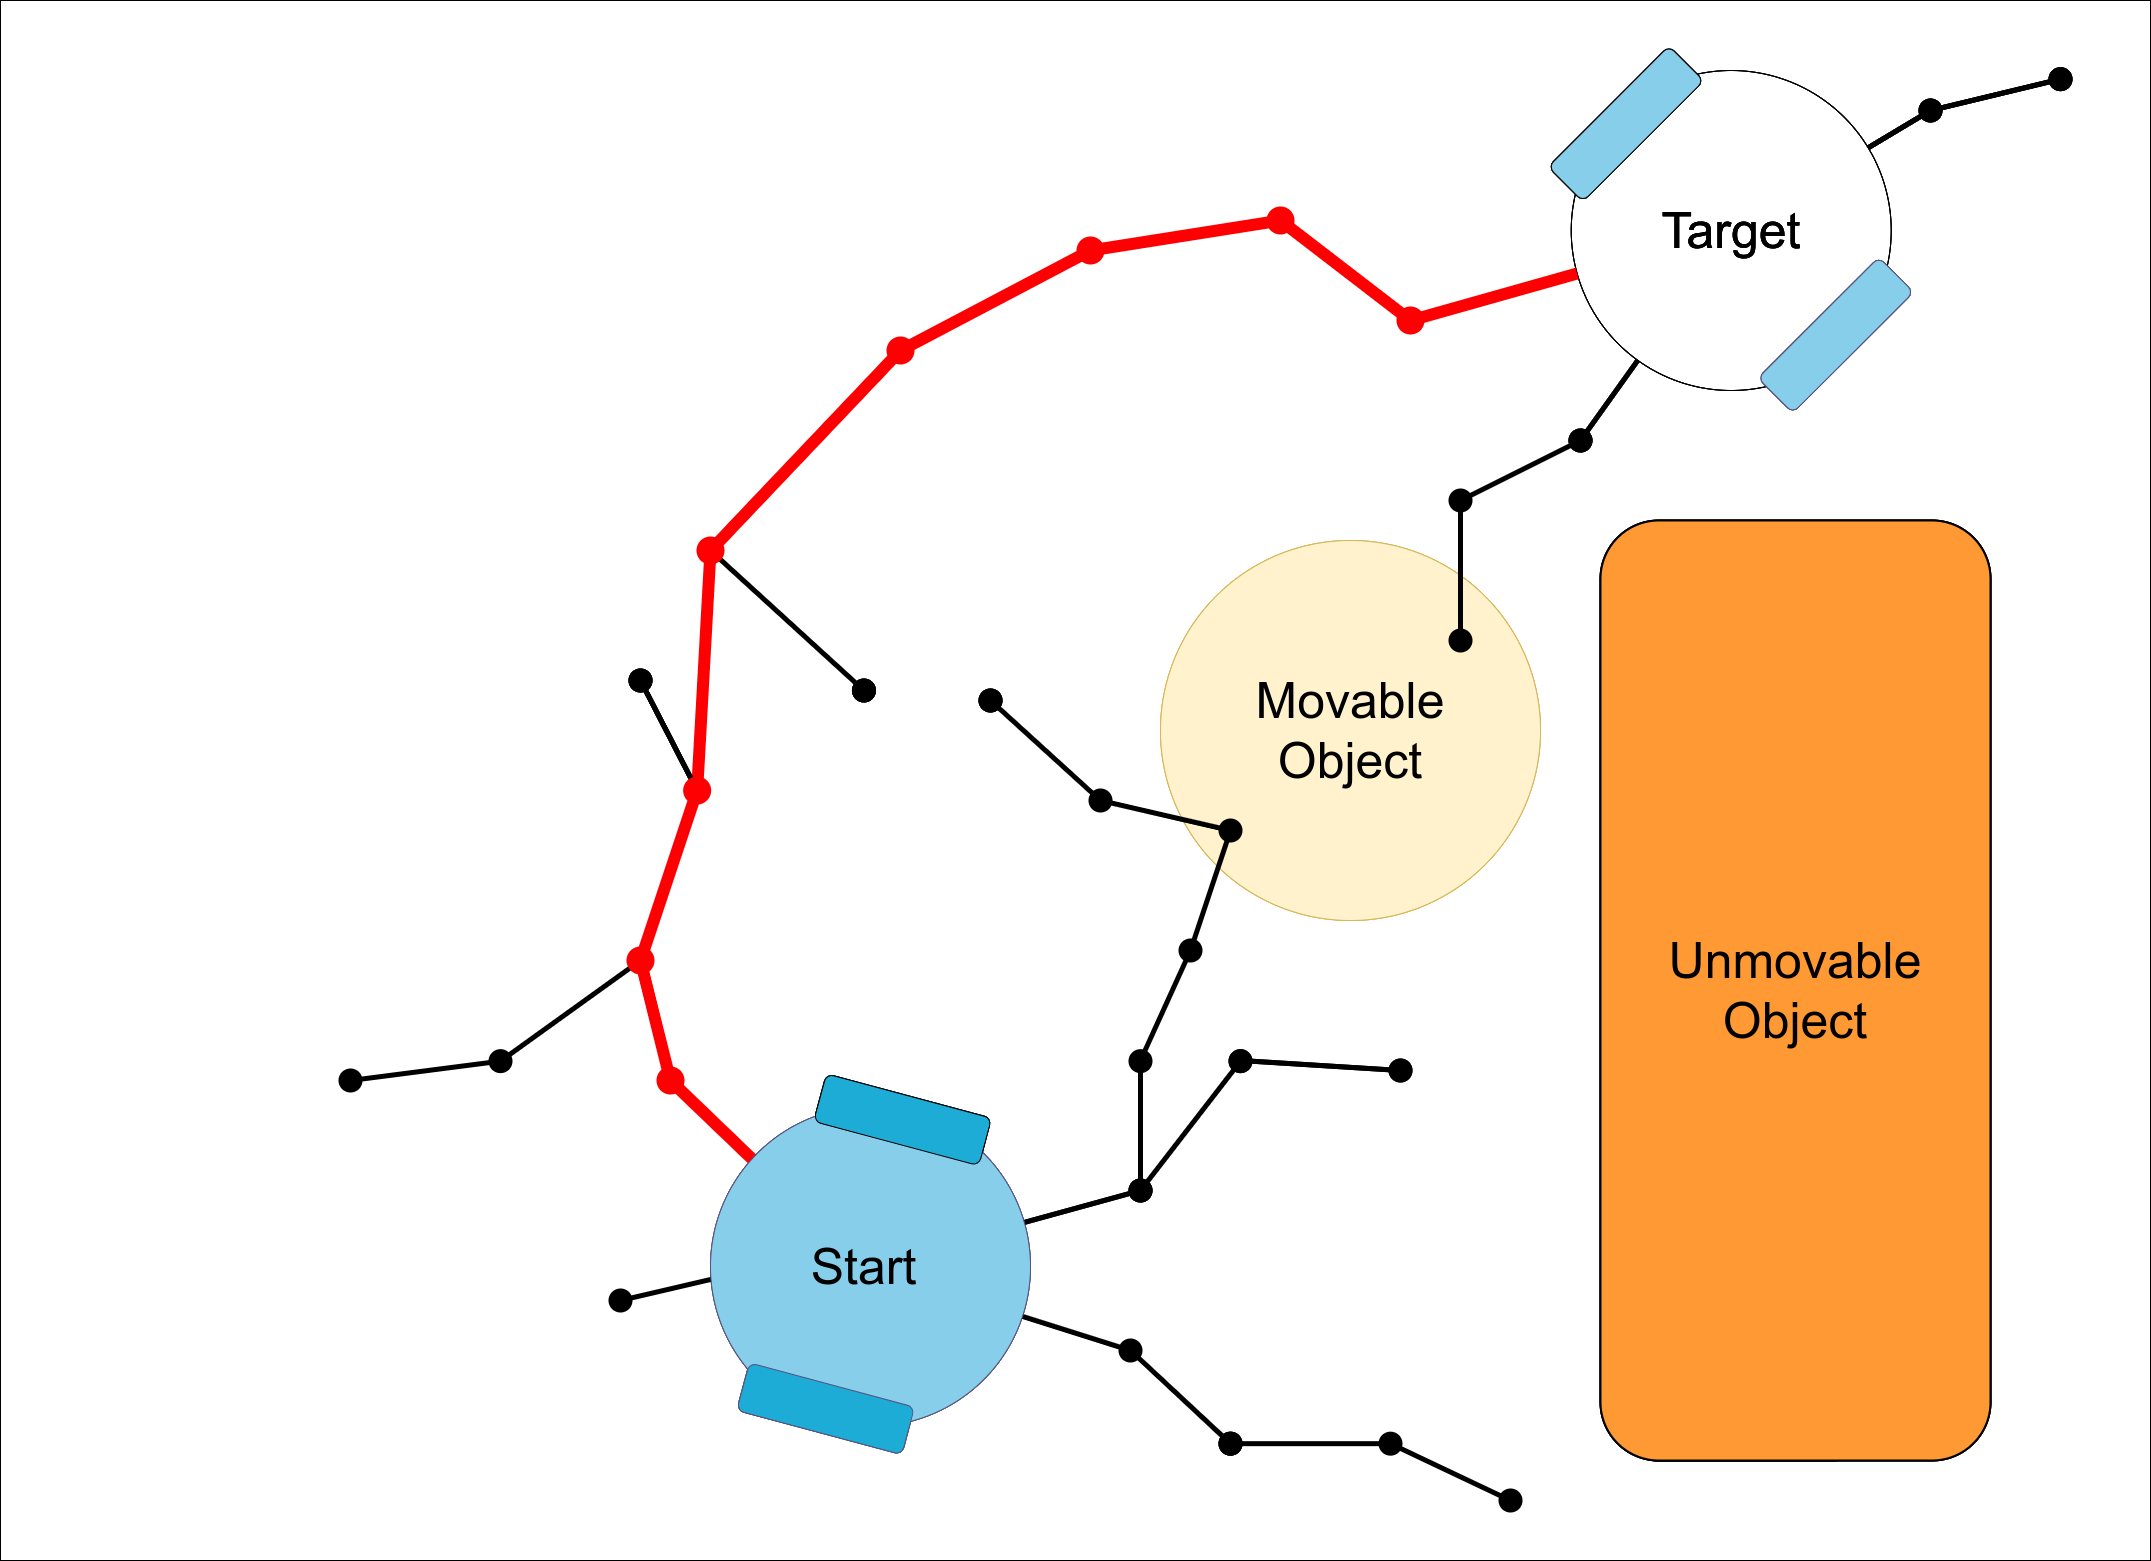
\includegraphics[width=1.10\textwidth]{figures/required_background/mp/7mp_path_found.drawio.png}
    \caption{Motion planner found a path found marked in red.}
    \end{subfigure}%

    \begin{subfigure}{\textwidth}
    \hspace{-0.7cm}
    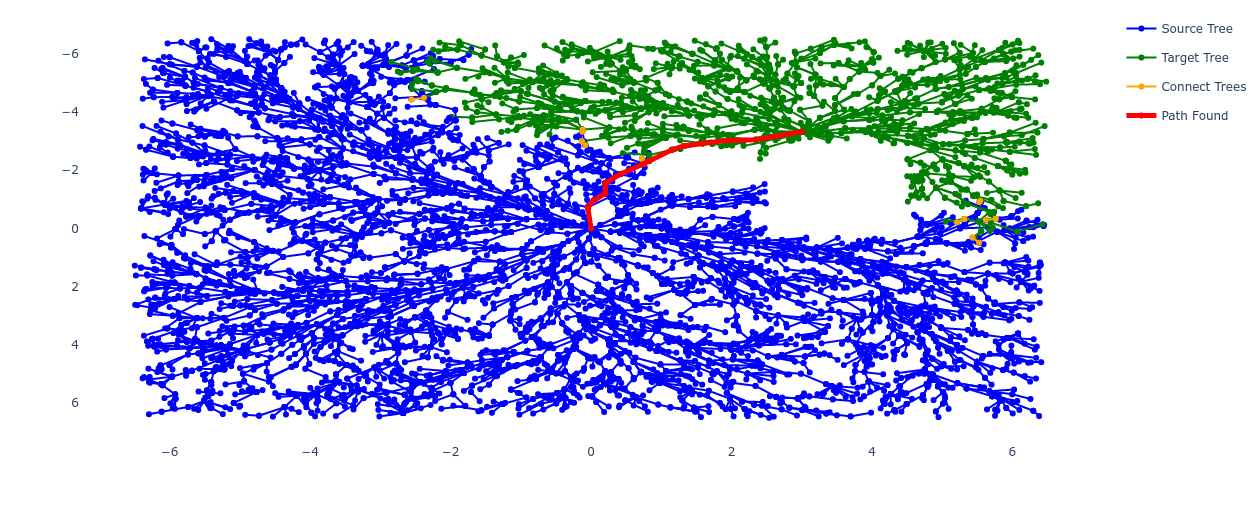
\includegraphics[width=1.1\textwidth]{figures/required_background/mp/mp_the_real_deal.png}
    \caption{A visualization of the implemented \acs{RRT*} algorithm\\when the stopping criteria was reached.}
    \end{subfigure}
    \label{fig:motion_planner_comparison}%
    \caption{Comparing schematic example to a visualization of the real algorithm.}
\end{figure}

The added fixed cost for a path crossing through a movable or unknown object motivates the motion planner to find the shortest path around objects but prefers moving an object over making a large detour. Tuning the additional fixed cost for a path crossing through movable or unknown space balances the robot's decision between how long of a detour the robot is willing to drive compared to pushing an object to free the path. Removing an unknown object bears more uncertainty compared to a movable object, which is why the additional cost to remove an unknown object is higher than the additional cost of a movable object. 

\begin{figure}[H]

    \centering
    \begin{subfigure}{\textwidth}
    \centering
    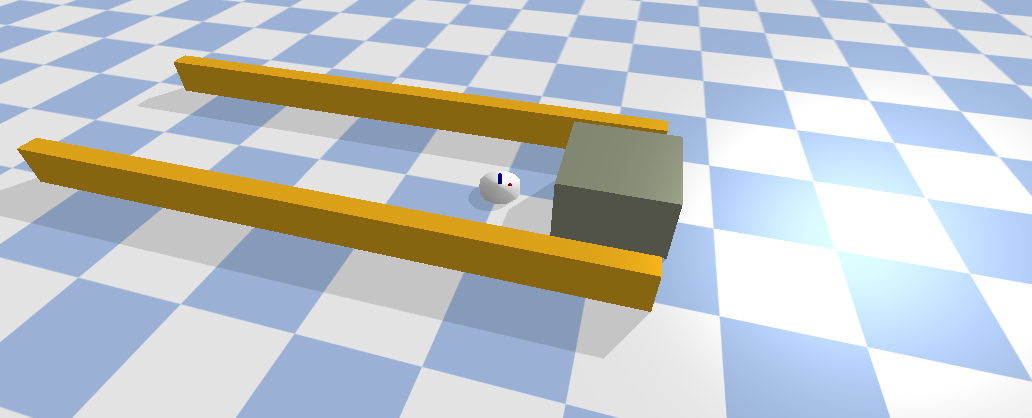
\includegraphics[width=0.9\textwidth]{figures/required_background/push_or_drive} \caption{Robot environment with the point robot, 2 yellow unmovable walls and an unknown brown box.}
    \end{subfigure}

    \begin{subfigure}{1.11\textwidth}
    \centering
    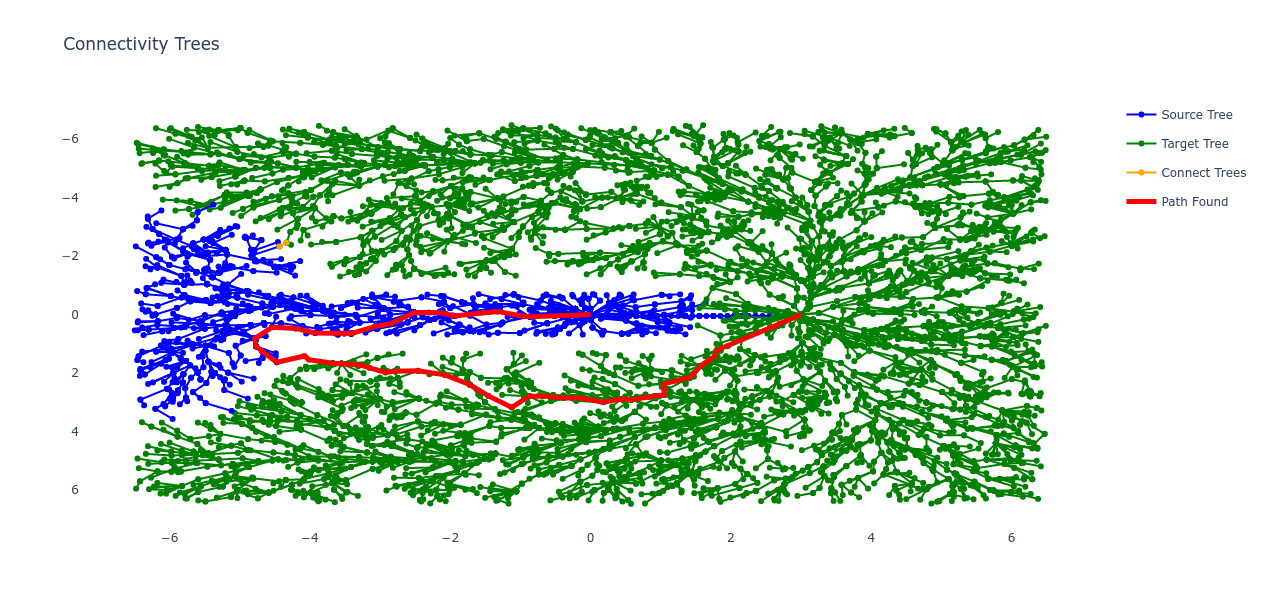
\includegraphics[width=\textwidth]{figures/required_background/mp/mp_high_fixed_cost}
    \caption{planned path around the brown box and yellow obstacles, with $\textrm{unknownSpaceCost} = 2$.}
    \end{subfigure}

    \begin{subfigure}{1.11\textwidth}
    \centering
    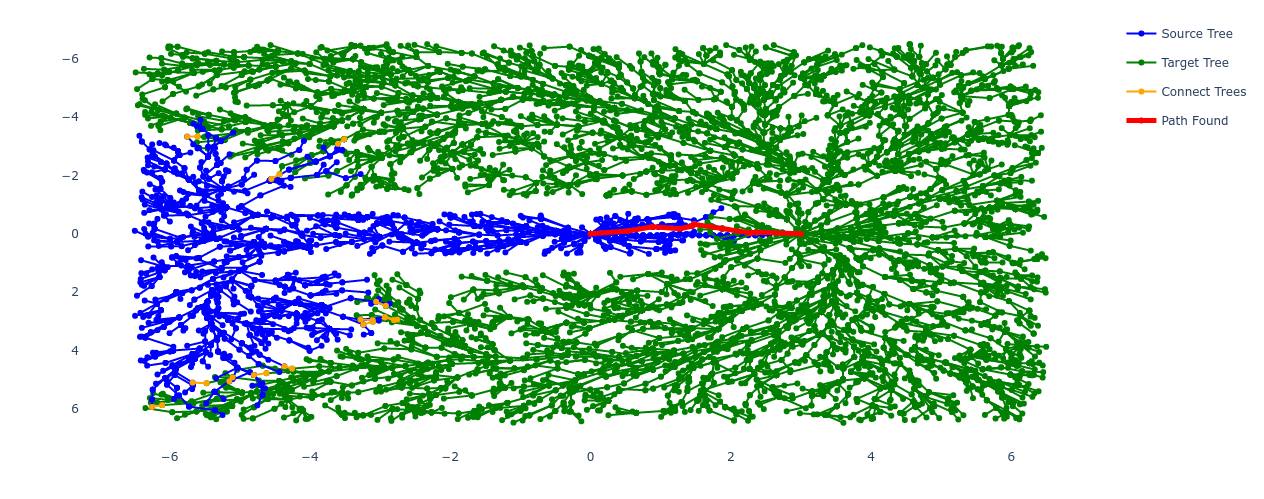
\includegraphics[width=\textwidth]{figures/required_background/mp/mp_low_fixed_cost}
    \caption{planned path going through the brown box, $\textrm{unknownSpaceCost} = 0.5$.}
    \end{subfigure}
    \caption{The robot tasked with driving toward the other side of the brown box.}%
    \label{fig:mp_push_or_drive}
\end{figure}

The proposed motion planning algorithm searches the configuration space from the start connectivity tree and the target connectivity tree. Exploring faster compared to the single tree \ac{RRT*} algorithm because two trees grow and explore faster than a single tree. The proposed algorithm rewires nodes, resulting in lowering the cost for existing paths, and converting to the optimal lowest-cost path with infinite sampling. System constraints are ensured by the \textit{ReachabilityCheck} that validates if a node is reachable from another node using system models.\bs

The proposed algorithm yields feasible paths (according to the system model used to check reachability) that respect the system constraints. The algorithm prevents planning a path through blocking objects except when no other option is available or it prevents a large detour. There are no performance tests taken on the modified motion planner other than visual inspection. For performance tests, and comparison with equivalent sample-based state-of-the-art motion planners see~\cite{chen_fast_2018}. Now that motion planning is discussed for drive actions, manipulation will be discussed for push actions.


\subsection{Manipulation Planning}%
\label{subsec:manipulation_planning}
With a push, two objects are primarily involved, the pushed object and the robot. Generally, and in this thesis, the pushed object's configuration is more important than the robots configuration. The robot is only a means to push the object toward the target configuration. At which final configuration the robot itself end up is of lesser importance. As long as during the push, the robot does not collide with objects other than the pushed object, and constraints on the robot must be respected.\bs

To plan a path that respects the constraints, the robots configuration is generated for every newly added sample in the manipulation planning algorithm. The \textit{ReachabilityCheck()} (see \Cref{table:functions_for_proposed_rrt_star} and line 33 in \Cref{pseudocode:proposed_rrt_star}) generates the robot configuration to validate if a new sample is reachable from an existing sample. This additional configuration is stored to create only feasible paths that respect the applied constraints. When the stopping criteria is reached and a shortest path is found, the generated robot configurations are discarded. \Cref{fig:manipulation_plannig_local_planner} displays a visual example of the procedure.\bs

\begin{figure}[H]
    \centering
    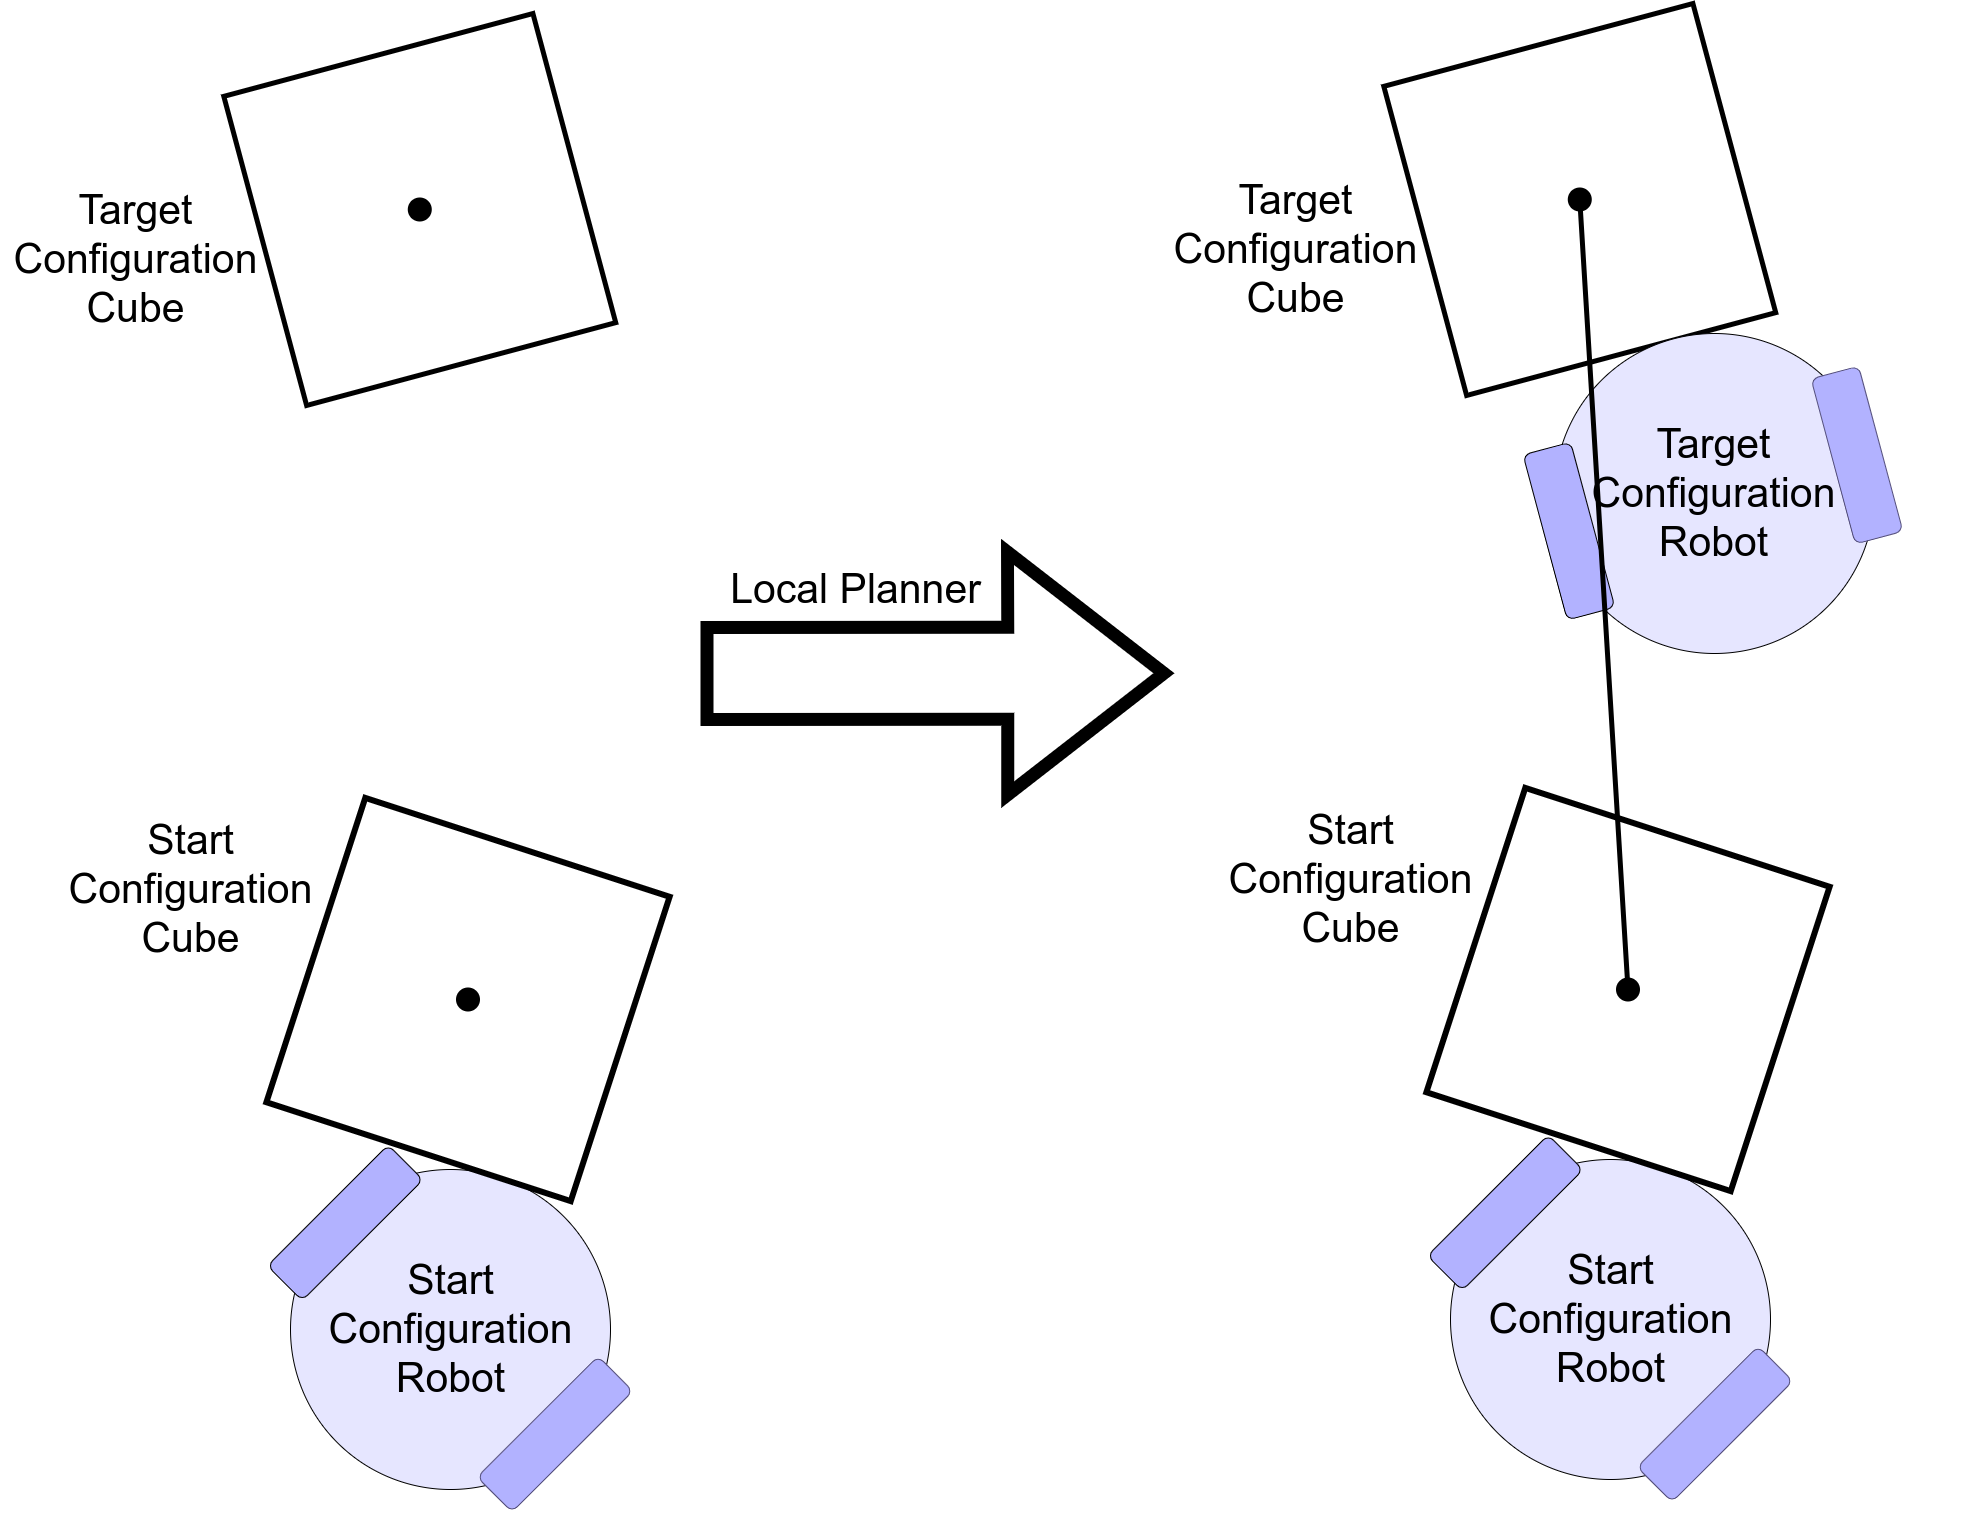
\includegraphics[width=0.6\textwidth]{figures/required_background/manipulation_local_planner}
    \caption{Generating a new robot configuration whilst adding a sample to the connectivity tree during manipulation planning.}%
    \label{fig:manipulation_plannig_local_planner}
\end{figure}

